%% ==========================================================================
%%  MILESTONE 3 --- FINAL PROJECT REPORT.  Due 6 November 2026.  Worth 15%.
%%
%%  Handout: "the complete source code; the final project report; and a final
%%  presentation.  Depending on logistics, the presentation may be conducted
%%  in person, online, or replaced by a 30-minute recorded presentation."
%%
%%  Shares preamble.tex and references.bib with survey.tex and midterm.tex,
%%  so notation and citations cannot drift.
%%
%%  CHANGED 2026-09-24, and the reasons are recorded rather than silent:
%%
%%  - This header used to say the survey's sections are reused wholesale and
%%    must not be forked. They cannot be reused as they stand: they call
%%    themselves "this survey" throughout and cross-reference sections only the
%%    survey has (sec:training, sec:retrieval, sec:taxonomy, sec:open:*), which
%%    would print as "??" here. Editing them is not an option either, since they
%%    are the source of the submitted Milestone 1 PDF. So every section below is
%%    a final_* or new file, and the survey's files are untouched.
%%
%%  - The stub carried "Do not start before the code freeze on 1 November".
%%    That gate predates the project running about five weeks ahead of the
%%    PHASES.md schedule, which itself wants a full draft by 30 October. The
%%    draft was written on 24 September, and the code freeze (task 5.2) now
%%    follows the draft instead of preceding it. Numbers written here are locked
%%    by the freeze, which tags the commit they come from.
%%
%%  - The byline listed four authors, including Aditya Anand, who dropped the
%%    course. It now matches the three-member roster of the submitted
%%    mid-term report (midterm_report.tex).
%%
%%  House style for every file this document inputs: no em dashes and no
%%  semicolons in prose (quotations, tables, TikZ and citation ranges exempt).
%%  Write .tex files with an editor, never a shell heredoc, which mangles
%%  backslashes.
%%
%%  Build:   mingw32-make report      (or, from report/: latexmk -pdf final.tex)
%%  Figures: mingw32-make figures     (generated, never committed or edited)
%% ==========================================================================
\documentclass[11pt]{article}
%% ==========================================================================
%%  preamble.tex --- packages, theorem environments, notation macros.
%%
%%  SHARED BY ALL THREE MILESTONE DOCUMENTS:
%%      survey.tex    Milestone 1, literature survey      (31 Aug 2026)
%%      midterm.tex   Milestone 2, per-member report      (12 Sep 2026)
%%      final.tex     Milestone 3, final report           ( 6 Nov 2026)
%%
%%  One preamble and one references.bib for the whole semester, so notation
%%  and citations cannot drift between documents.  If you need a symbol,
%%  add it HERE -- never redefine it inside a section file.
%% ==========================================================================

% ---------- page geometry & fonts -----------------------------------------
\usepackage[letterpaper,margin=1in]{geometry}
% Palatino text + matching math.  newpx is built on TeX Gyre Pagella, so it
% needs no URW base-35 fonts -- which a minimal TinyTeX install does not ship.
% If newpx is unavailable, `mathpazo' is the drop-in substitute wherever the
% URW fonts *are* present.
\usepackage[T1]{fontenc}
\usepackage[utf8]{inputenc}
\usepackage{newpxtext}
\usepackage{microtype}

% ---------- mathematics ---------------------------------------------------
% Order matters: amsmath must be loaded before newpxmath.
\usepackage{amsmath,amssymb,amsthm,mathtools}
\usepackage{newpxmath}
\usepackage{stmaryrd}          % \llbracket \rrbracket -- secret-sharing brackets

% ---------- floats, tables, algorithms ------------------------------------
\usepackage{booktabs}
\usepackage{multirow}
\usepackage{longtable}
\usepackage{array}
\usepackage{graphicx}
\graphicspath{{figures/}}
\usepackage{algorithm}
\usepackage[noend]{algpseudocode}
\floatname{algorithm}{Algorithm}
\usepackage{tikz}
\usetikzlibrary{arrows.meta,positioning,fit,backgrounds,calc,decorations.pathreplacing}

% ---------- colour & links ------------------------------------------------
\usepackage{xcolor}
\definecolor{CiteGreen}{RGB}{0,120,60}
\definecolor{LinkRed}{RGB}{160,20,20}
\definecolor{UrlBlue}{RGB}{20,60,170}
\definecolor{DraftOrange}{RGB}{200,90,0}
\usepackage[
  colorlinks=true,
  citecolor=CiteGreen,
  linkcolor=LinkRed,
  urlcolor=UrlBlue,
  bookmarksnumbered=true
]{hyperref}
\usepackage{cleveref}

% ==========================================================================
%  Theorem environments.  One counter runs through
%  Definition/Theorem/Lemma/Proposition/Observation; Claim has its own.
% ==========================================================================
\theoremstyle{plain}
\newtheorem{theorem}{Theorem}[section]
\newtheorem{lemma}[theorem]{Lemma}
\newtheorem{proposition}[theorem]{Proposition}
\newtheorem{corollary}[theorem]{Corollary}
\newtheorem{definition}[theorem]{Definition}
\newtheorem{observation}[theorem]{Observation}
\newtheorem{conjecture}[theorem]{Conjecture}
\newtheorem{claim}{Claim}[section]

\theoremstyle{definition}
\newtheorem{example}[theorem]{Example}
\newtheorem{remark}[theorem]{Remark}
\theoremstyle{plain}

% NOTE.  cleveref cannot tell these apart --- they share the `theorem'
% counter, so \Cref would call every one of them "Theorem".  Write
% `Remark~\ref{...}', `Example~\ref{...}' explicitly.  \Cref is safe for
% sections, figures and tables.

% Bold, unpunctuated "Proof" head (amsthm defaults to italic "Proof.").
\makeatletter
\renewenvironment{proof}[1][\proofname]{\par
  \pushQED{\qed}%
  \normalfont \topsep6\p@\@plus6\p@\relax
  \trivlist
  \item[\hskip\labelsep\bfseries #1\@addpunct{}]\ignorespaces
}{%
  \popQED\endtrivlist\@endpefalse
}
\makeatother

% ==========================================================================
%  Draft notes.  Flip to \draftfalse for a clean submission copy; nothing
%  else in the document changes.
%
%      \todo{...}    something still to be written
%      \verify{...}  a claim that must be checked against the paper
%      \gap{...}     a place where the survey must argue the gap explicitly
%
%  Before submitting, find what is outstanding:
%      grep -rn '\\todo{\|\\verify{\|\\gap{' sections/ *.tex
% ==========================================================================
\newif\ifdraft
% Flipped for the Milestone 1 submission copy, 2026-09-03. Nothing currently
% renders differently, since no live \todo/\verify/\gap remains in any section
% that survey.tex inputs, but the submitted PDF should not be a draft build.
\draftfalse

\newcommand{\draftnote}[1]{%
  \ifdraft{\color{DraftOrange}\sffamily\small[\,#1\,]}\fi}
\newcommand{\todo}[1]{\draftnote{\textbf{TODO:} #1}}
\newcommand{\verify}[1]{\draftnote{\textbf{VERIFY:} #1}}
\newcommand{\gap}[1]{\draftnote{\textbf{GAP-ARGUMENT:} #1}}

% ==========================================================================
%  PROJECT NOTATION.
%
%  Fixed here, once, for all three documents.  Follows [NUDGE] where the two
%  base papers disagree, since its notation is the more standard.  Do not
%  introduce a competing symbol in a section file --- add it here instead,
%  and say so at the weekly sync so nobody duplicates it.
% ==========================================================================

% ---- parties and sharing -------------------------------------------------
\newcommand{\party}[1]{P_{#1}}                 % server P_0, P_1, P_2
\newcommand{\shr}[1]{\llbracket #1 \rrbracket} % replicated / additive sharing
\newcommand{\ring}{\mathcal{R}}                % the ring Z_{2^b}
\newcommand{\Ztwo}[1]{\mathbb{Z}_{2^{#1}}}
\newcommand{\bits}{b}                          % ring bit-length
\newcommand{\fracbits}{t}                      % fixed-point fractional bits
\newcommand{\seclen}{\lambda}                  % PRF seed / security parameter

% ---- the recommendation problem -----------------------------------------
\newcommand{\users}{m}                         % number of users
\newcommand{\items}{n}                         % number of items
\newcommand{\dime}{d}                          % embedding dimension
\newcommand{\iters}{\ell}                      % power-iteration rounds
\newcommand{\topk}{k}                          % recommendations returned
\newcommand{\ratings}{\mathbf{U}}              % user-item rating matrix, m x n
\newcommand{\userembed}{\mathbf{A}}            % user embeddings, m x d (SECRET)
\newcommand{\itemembed}{\mathbf{B}}            % item embeddings, d x n (PUBLIC)
\newcommand{\uvec}[1]{\mathbf{u}^{(#1)}}       % user i's rating vector
\newcommand{\avec}[1]{\mathbf{a}^{(#1)}}       % user i's embedding

% ---- protocols -----------------------------------------------------------
\DeclareMathOperator{\Trunc}{Trunc}
\DeclareMathOperator{\ApproxNormalize}{ApproxNormalize}
\DeclareMathOperator{\ApproxFactor}{ApproxFactor}
\DeclareMathOperator{\SetOrthogonal}{SetOrthogonal}
\DeclareMathOperator{\Normalize}{Normalize}
\DeclareMathOperator{\Gen}{Gen}
\DeclareMathOperator{\Eval}{Eval}
\DeclareMathOperator{\EvalFull}{EvalFull}
\newcommand{\dpf}{\mathrm{DPF}}
\newcommand{\fss}{\mathrm{FSS}}

% ---- ideal functionalities (final report, section 2) ---------------------
%  REQUIREMENTS.md section 3.2 defines F_train and F_serve. F_train^leaky is
%  the weaker functionality docs/threat-model.md section 8.4 introduces for
%  the normaliser that opens ||v||.
\newcommand{\Ftrain}{\mathcal{F}_{\mathrm{train}}}
\newcommand{\Fleaky}{\mathcal{F}_{\mathrm{train}}^{\mathrm{leaky}}}
\newcommand{\Fserve}{\mathcal{F}_{\mathrm{serve}}}
\newcommand{\Sim}{\mathcal{S}}

% ---- shorthand for the two base papers ----------------------------------
%  Use \pirsona and \nudge in prose so the naming stays uniform; the macros
%  cite as well as name, so `\nudge{} publishes $\itemembed$ in the clear'
%  produces both the name and the citation.
\newcommand{\pirsona}{\textsc{Pirsona}\,\cite{pirsona2021}}
\newcommand{\nudge}{\textsc{Nudge}\,\cite{nudge2026}}
\newcommand{\pirsonaplain}{\textsc{Pirsona}}
\newcommand{\grotto}{\textsc{Grotto}\,\cite{grotto2023}}
\newcommand{\grottoplain}{\textsc{Grotto}}
\newcommand{\duoram}{\textsc{Duoram}\,\cite{duoram2023}}
\newcommand{\duoramplain}{\textsc{Duoram}}
\newcommand{\prac}{\textsc{Prac}\,\cite{prac2024}}
\newcommand{\pracplain}{\textsc{Prac}}
\newcommand{\floram}{\textsc{Floram}\,\cite{floram2017}}
\newcommand{\tiptoe}{\textsc{Tiptoe}\,\cite{tiptoe2023}}
\newcommand{\pacmann}{\textsc{Pacmann}\,\cite{pacmann2025}}
\newcommand{\compass}{\textsc{Compass}\,\cite{compass2025}}
\newcommand{\panther}{\textsc{Panther}\,\cite{panther2025}}
\newcommand{\wally}{\textsc{Wally}\,\cite{wally2024}}
\newcommand{\sanns}{\textsc{Sanns}\,\cite{sanns2020}}
\newcommand{\tiptoeplain}{\textsc{Tiptoe}}
\newcommand{\pacmannplain}{\textsc{Pacmann}}
\newcommand{\compassplain}{\textsc{Compass}}
\newcommand{\pantherplain}{\textsc{Panther}}
\newcommand{\wallyplain}{\textsc{Wally}}
\newcommand{\sannsplain}{\textsc{Sanns}}
\newcommand{\floramplain}{\textsc{Floram}}
\newcommand{\nudgeplain}{\textsc{Nudge}}
\newcommand{\sys}{\textsc{OblivRec}}           % our system, working name

% ---- generic -------------------------------------------------------------
\newcommand{\N}{\mathbb{N}}
\newcommand{\R}{\mathbb{R}}
\newcommand{\Z}{\mathbb{Z}}
\newcommand{\set}[1]{\left\{#1\right\}}
\newcommand{\abs}[1]{\left\lvert#1\right\rvert}
\newcommand{\norm}[1]{\left\lVert#1\right\rVert}
\newcommand{\inner}[2]{\left\langle #1, #2 \right\rangle}
\DeclareMathOperator*{\argmax}{arg\,max}
\DeclareMathOperator*{\argmin}{arg\,min}
\DeclareMathOperator{\poly}{poly}


\begin{document}

\title{\bfseries \sys: Privacy-Preserving Recommendation\\
       with Private Training and Private Delivery}

% \author{Mainak Sarkar (230619) \and Shrasti Dwivedi (230982) \and
%         Aditya Anand (230065) \and Shravan Agrawal (230984)}
\author{Mainak Sarkar (230619) \and Shrasti Dwivedi (230982) \and
        Shravan Agrawal (230984)}

\date{CS670: Cryptographic Techniques for Privacy Preservation\\
      Indian Institute of Technology Kanpur \\
      6 November 2026}

\maketitle

%% ==========================================================================
%%  FINAL REPORT --- ABSTRACT
%%
%%  House style for every final_* file and every file final.tex inputs: no em
%%  dashes and no semicolons in prose. Quotations, table cells, TikZ and
%%  citation ranges are exempt. Written with the Write/Edit tools only.
%% ==========================================================================
\begin{abstract}
\noindent
A recommender learns from what its users consume, so a private recommender has
to protect two things: the ratings the model is trained on, and the items a
user fetches once the recommendations arrive. \nudgeplain{}, the strongest
recent system for the first, trains a matrix factorisation across three servers
under replicated secret sharing, publishes the item embeddings in the clear, and
leaves the fetch to ``other means''. \pirsonaplain{} fetches privately but
trains with four parties over a Boolean circuit.

We build \sys{}, the composition of the two: \nudgeplain{}'s power-iteration
training under 2-of-3 replicated sharing, followed by two-server private
information retrieval from a distributed point function, with one implementation
of that function serving both the training protocol's comparison gate and the
read. On MovieLens-100K, composing costs exactly the sum of the two halves, to
the byte. The spec-faithful normaliser, which reveals nothing, costs between
0.0018 and 0.0041 of nDCG@20 against one that reveals a norm, and 5.3 times the
rounds. Truncation, not the comparison gate, is where the rounds go. Without the
private read, ten observed fetches recover a user's private embedding to a cosine
of 0.84, and neither decoy traffic nor \nudgeplain{}'s own differential privacy
brings the attack down to what popularity alone achieves.

We also report where the composition is weaker than its parts. On a wide-area
link, downloading the whole catalogue beats our unbatched private read by a
factor of 4.6. Until we added a one-round check, a malicious client could cast a
vote of arbitrary weight in the next model, and sixteen such clients destroyed
it. The check stops inflated weight but not a forged key that redistributes it.
Security is semi-honest with at most one corrupted server, and it is argued by a
simulation sketch, not proven.
\end{abstract}


\tableofcontents
\newpage

% --------------------------------------------------------------------------
%  1  Introduction and motivation
%% ==========================================================================
%%  FINAL REPORT --- SECTION 1, INTRODUCTION
%%  Self-contained: the survey's introduction.tex describes the survey and is
%%  left untouched, since it is the source of a submitted document.
%% ==========================================================================
\section{Introduction}
\label{sec:intro}

A recommender system is built from the most revealing data its users produce:
what they watched, read and bought. That this data is identifying, and not
merely sensitive, was shown by Narayanan and Shmatikov~\cite{narayanan2008}, who
matched records in the anonymised Netflix Prize dataset to public profiles and
report ``uncovering their apparent political preferences and other potentially
sensitive information''. A recommender that its operator cannot read therefore
has to protect more than one thing. It has to protect the ratings the model is
trained on, and it has to protect what the user does with the recommendations
afterwards, because fetching a recommended item says which item it was.

\subsection{Two papers, two halves}
\label{sec:intro:gap}

The course handed us two systems that each address one of these. \nudge{}
trains a matrix factorisation of the rating matrix across three servers, at most
one of them compromised, under 2-of-3 replicated secret sharing. Its central
observation is that a matrix--vector product under this sharing costs
communication proportional to the output vector rather than to the matrix, so an
algorithm written as a chain of such products with a few non-linear steps
between them is cheap. Power iteration has that shape. \nudgeplain{} publishes
the resulting item embeddings $\itemembed$ in the clear, by design, and computes
each user's scores in shared form. It then stops, and says so: the system
``relies on other means (e.g., Apple's private relay, Tor, or cryptographic
private information retrieval) to let users fetch data items in a private
way''~\cite{nudge2026}.

\pirsona{} addresses the fetch. Users retrieve items by multi-server private
information retrieval (PIR), and the servers harvest a secret-shared record of
what each user consumed directly from the PIR queries, so the next round of
training needs no separate upload. Its training core is a ``carefully optimized
4PC Boolean matrix factorization'', and its authors are explicit that they
``opted for the most performant primitives available (at the expense of rather
strong non-collusion assumptions)''~\cite{pirsona2021}.

Neither paper builds both halves well, and neither measures what happens when
they meet. That meeting point is where this project sits. \nudgeplain{}'s public
$\itemembed$ is a complete latent-factor model of the catalogue, known to
everyone, so a fetch observed in the clear is not an isolated fact about a user.
It is a projection of that user's private embedding onto a basis the observer
already holds. Section~\ref{sec:leak} measures how quickly those projections
give the user away.

\subsection{What we built and what we found}
\label{sec:intro:contrib}

\sys{} is the composition: \nudgeplain{}'s training core, followed by
two-server PIR built from a distributed point function (DPF), with
\pirsonaplain{}'s harvest connecting delivery back to training. Everything
cryptographic is written from scratch in C++17, including the DPF, which serves
both as the read layer and as the comparison gate inside training. Our
contributions are these.

\begin{enumerate}
  \item \textbf{A working composition.} Private training runs end to end on
    MovieLens-100K, the trained model is served from three separate server
    processes over TCP, and each recommended record is fetched by DPF-PIR and
    checked byte for byte against a cleartext lookup
    (Sections~\ref{sec:design} and~\ref{sec:impl}).

  \item \textbf{The cost of the composition, measured half by half.} Composing
    costs exactly the sum of the halves, which the benchmark asserts to the
    byte. \nudgeplain{}'s Theorem~4.2 is measured rather than quoted:
    quadrupling the input matrix raises traffic by 4.4\% and leaves the round
    count unchanged. Truncation accounts for 68.6 to 74.4\% of all rounds, and
    the FSS comparison gate for 3.1\%. A normaliser that reveals nothing costs
    between 0.0018 and 0.0041 of nDCG@20 and 5.3 times the rounds, and it
    cannot run in a 64-bit ring at all (Section~\ref{sec:eval}).

  \item \textbf{Why the fetch must be private, and why cheaper defences fail.}
    Ten observed fetches recover a user's private embedding to a cosine of
    0.84, well above a popularity control. Decoy traffic at five times the
    real volume leaves the attack far above that control, and \nudgeplain{}'s
    own differential-privacy mechanism makes the attack stronger while
    removing 71\% of recommendation quality. We reconcile that figure with
    \nudgeplain{}'s own 17\% (Section~\ref{sec:leak}).

  \item \textbf{A malicious-client hole in the composition, and its partial
    fix.} The harvest path accepted a vote of any weight. We measure what that
    buys an attacker, close weight inflation with a one-round check, show by
    construction what the check does not close, and measure the
    denial-of-service amplification that full-domain evaluation invites
    (Section~\ref{sec:leak:malicious}).

  \item \textbf{A stated security argument.} A threat model with six adversary
    classes, a leakage profile, and a real/ideal simulation sketch that walks
    every message. The sketch shows that one of our two normalisers is not
    simulable against the intended functionality, and we say which numbers
    came from it (Section~\ref{sec:threat}).
\end{enumerate}

We also report results that go against us, because a reader deciding whether to
build this needs them. On a wide-area link, downloading the entire catalogue
beats our private read by a factor of 4.6, since delivery costs one round trip
per recommendation and we did not batch them. The spec-faithful normaliser loses
most of its quality at a single power iteration. And one bug, a silently
clamping comparison range, would have been reported as ``privacy costs 24\% of
recommendation quality'' had we measured only cost.

\paragraph{What this report does not claim.} Security is semi-honest, and two
colluding servers learn everything. The evaluation runs on MovieLens-100K, not
on MovieLens-1M or Netflix scale. Wide-area profiles are emulated at the channel
level, not with kernel network emulation. The security argument is a sketch.
Section~\ref{sec:limits} states each of these in full.

\subsection{Organisation}
\label{sec:intro:org}

Section~\ref{sec:threat} fixes the threat model and the security argument.
Section~\ref{sec:background} covers the primitives, and
Section~\ref{sec:design} the system design. Section~\ref{sec:impl} describes the
implementation and how it was verified, and Section~\ref{sec:eval} evaluates its
cost and quality. Section~\ref{sec:leak} measures what the composition leaks and
what a malicious client can do. Section~\ref{sec:related} places the work,
Section~\ref{sec:limits} lists its limitations, and
Section~\ref{sec:conclusion} concludes. Appendix~\ref{app:protocols} gives the
protocols as pseudocode, and Appendix~\ref{app:reproduce} maps every figure to
the command and the data file that produce it.

%  2  Threat model and security
%% ==========================================================================
%%  FINAL REPORT --- SECTION 2, THREAT MODEL AND SECURITY
%%  Source: docs/threat-model.md sections 1-3, 5, 7 and 8, and
%%  REQUIREMENTS.md section 3.2 for the ideal functionalities.
%% ==========================================================================
\section{Threat model and security}
\label{sec:threat}

This section says what \sys{} protects, against whom, and how far the argument
for it goes. It comes before the design on purpose: every later section is read
against it, and the most important sentences in this report are the ones that
say what is \emph{not} protected.

\subsection{Setting}
\label{sec:threat:setting}

There are three servers $\party{0}, \party{1}, \party{2}$, run by independent
operators, and $\users$ users. The rating matrix $\ratings \in \R^{\users \times
\items}$ is held in 2-of-3 replicated secret shares, so no single server holds
it. Training produces an item-embedding matrix $\itemembed \in \R^{\dime \times
\items}$, which is opened to everyone, and user embeddings $\userembed \in
\R^{\users \times \dime}$, which stay shared. Opening $\itemembed$ is
\nudgeplain{}'s design and not an oversight: each converged row is revealed
before the next is computed, which is what keeps orthogonalisation cheap.

To be served, user $i$ asks each server for its share of the score vector
$\avec{i}\itemembed$, reconstructs it, and selects the top $\topk$ items
\emph{on the user's own machine}. The user then fetches each of the $\topk$
records by two-server DPF-PIR against $\party{0}$ and $\party{1}$. The catalogue
of records is public, and all three servers hold it.

\subsection{Ideal functionalities}
\label{sec:threat:ideal}

Two functionalities describe what the system is meant to compute and to whom
each output goes. They are taken from the project's requirements document.
%
\begin{align*}
  \Ftrain(\shr{\ratings}, \dime, \iters)\colon\quad
    & (\userembed, \itemembed) \gets \ApproxFactor(\ratings) \text{ by $\iters$
      power iterations per component,}\\
    & \text{every server receives $\itemembed$ in the clear and its shares of
      $\shr{\userembed}$.}\\[4pt]
  \Fserve(\shr{\avec{i}}, \itemembed, \topk)\colon\quad
    & \mathbf{s} \gets \avec{i}\itemembed, \quad
      \mathbf{s}[j] \gets -\infty \text{ for every item $j$ user $i$ has
      rated},\\
    & T \gets \text{the top-$\topk$ indices of } \mathbf{s},\\
    & \text{the user receives $T$ and the records $D[T]$, and the servers
      receive nothing.}
\end{align*}
%
The second line of $\Fserve$'s output is what \sys{} adds to \nudgeplain{}. A
third functionality is needed because of one of our two normalisers, and
Section~\ref{sec:threat:gaps} explains why: $\Fleaky$ is $\Ftrain$ with the
sequence of norms $\{\norm{\mathbf{v}}\}$ from every normalisation added to the
servers' output.

\subsection{Adversary classes}
\label{sec:threat:classes}

Table~\ref{tab:adversaries} lists six classes. The headline guarantee is against
\textbf{A1}, one semi-honest server, which is exactly \nudgeplain{}'s model.

\begin{table}[t]
\centering
\small
\caption{Adversary classes and what \sys{} guarantees against each. A3 is the
assumption the whole system rests on.}
\label{tab:adversaries}
\begin{tabular}{@{}l p{3.6cm} p{9.2cm}@{}}
\toprule
 & Adversary & Guarantee \\
\midrule
A1 & One semi-honest server & Nothing is learned beyond the leakage profile of
  Section~\ref{sec:threat:leakage}. Argued by the sketch in
  Section~\ref{sec:threat:sketch}. \\
A2 & One semi-honest server and colluding users & Honest users' ratings stay
  hidden. Model \emph{quality} is not protected: colluding clients can distort
  the harvested training input (Section~\ref{sec:leak:malicious}). \\
A3 & Two or more colluding servers & \textbf{No guarantee.} Any two servers hold
  all three shares and reconstruct everything, and the two PIR servers together
  reconstruct every fetched index. \\
A4 & A malicious (deviating) server & Out of scope, as in \nudgeplain{}. A
  deviating server can corrupt correctness and availability. \\
A5 & A malicious user & Retrieval corrupts only that user's own output. The
  harvest path accepted a vote of any weight, which we close for inflation but
  not for redistribution, and full-domain evaluation is an unmitigated
  denial-of-service lever (Section~\ref{sec:leak:malicious}). \\
A6 & A network observer & Sees message sizes and timing. Sizes depend only on
  public parameters, measured in Section~\ref{sec:eval:wire}. Server-side timing
  is bounded in Section~\ref{sec:eval:timing}, and wire timing is not
  analysed. \\
\bottomrule
\end{tabular}
\end{table}

\subsection{Leakage profile}
\label{sec:threat:leakage}

\paragraph{Hidden from any single server.} Individual ratings, and which items a
user rated. The user embeddings $\userembed$. Each score vector, and the top-$k$
indices chosen from it. Which records a user fetches.

\paragraph{Leaked by design.} The parameters $\users, \items, \dime, \iters,
\topk, \bits, \fracbits$. The item-embedding matrix $\itemembed$, in the clear.
The number of non-zero ratings, which the truncation schedule uses as a public
bound and which \nudgeplain{} also leaks, unless every user is made to submit a
fixed number of ratings at a cost in quality. How many queries each user makes,
and when.

\paragraph{Outside the protocol's protection.} Correlation between when a user
queries and external events. Anything an adversary can infer from $\itemembed$
together with an observed fetch, which is precisely why the fetch has to be
private and is the subject of Section~\ref{sec:leak}.

\subsection{A real/ideal simulation sketch}
\label{sec:threat:sketch}

The claim, for class A1, is that for each corrupted server $\party{c}$ there is
a simulator $\Sim_c$ which, given only $\party{c}$'s input shares and the output
the functionality declares for it, produces a transcript computationally
indistinguishable from $\party{c}$'s real view. That view is its input shares,
its pseudorandom-function keys, its local randomness, and every ring element it
receives. We argue it step by step against the code. This is a \emph{sketch}.
There is no formal security parameter, no reduction, and no written hybrid
argument, and the three servers are not symmetric, since only $\party{0}$ and
$\party{1}$ hold DPF keys and the truncation protocol rotates a helper role. So
``by symmetry'' is never used.

\paragraph{The substrate.} A value is shared as $x = x_0 + x_1 + x_2$ with party
$i$ holding $(x_i, x_{i+1})$. Any two of three shares of a 3-out-of-3 additive
sharing are uniform and independent of $x$, so $\Sim_c$ samples two uniform ring
elements per value and never needs $\ratings$. Correlated randomness comes from
pairwise PRF keys. Party $i$ derives $\alpha_i = F(k_i, \mathit{ctr}) - F(k_{i-1},
\mathit{ctr})$, and the three sum to zero with no communication. $\party{c}$ can
compute its own $\alpha_c$ but no other party's, because each needs a key it
does not hold. That asymmetry is what makes every incoming element below
uniform.

\paragraph{Matrix--vector products.} Each party computes its share of the product
locally, masks it with $\alpha_i$, and sends one ring element per output entry.
$\party{c}$ receives $z_{c+1}$, masked by $\alpha_{c+1}$, which uses a key
$\party{c}$ lacks, so $\Sim_c$ samples it uniformly. The message size is set by
the public output length alone.

\paragraph{Truncation.} A helper $h$ supplies a correlated pair $(r, r \gg t)$
and the other two parties open $c = x - r$ and reshare. There are two cases. If
$\party{c}$ is an opener, it sees $x - r$ with $r$ uniform and known only to
$h$, so $\Sim_c$ samples $c$ uniformly. If $\party{c}$ is the helper, it sees
only the pair it generated, and the reshare is masked with a pairwise secret it
does not hold, so $\Sim_c$ replays its own randomness and samples the rest. A
party that held $r$ and also saw $x - r$ would recover $x$, which is why the
helper is passed explicitly at every call site.

\paragraph{Normalisation.} For the spec-faithful \texttt{FssNormalizer}, the
comparison gate opens $S + r$ where $r$ is drawn from a range $\kappa = 40$ bits
wider than $S$, so the opening is statistically close to uniform and $\Sim_c$
samples it. The DCF evaluations are local, and the Newton iterations are
multiplications and truncations already covered.

\paragraph{Orthogonalisation.} Entirely local, because every product is a share
times a public row of $\itemembed$. Nothing is sent.

\paragraph{Opening each row of $\itemembed$.} $\itemembed$ is $\Ftrain$'s
declared output, so $\Sim_c$ is given it and replays it. This step is free in the
simulation and is also the largest leakage surface in the system. That is not a
contradiction. It is leakage by design, and Section~\ref{sec:leak:attack} is the
measurement of what it costs.

\paragraph{Serving.} Scores are a public matrix applied to a shared vector, so
every server computes its share locally and sends it to the user, not to another
server. The seen-item mask arrives from the user as a share, which $\Sim_c$
samples.

\paragraph{Delivery.} $\party{c} \in \{\party{0}, \party{1}\}$ receives one DPF
key per fetch. A single key is pseudorandom and independent of the index by the
DPF's security, so $\Sim_c$ samples a key of the right length, 227 bytes at 11
domain bits. The server then expands the key over the whole domain and takes an
inner product with every record, so the work does not depend on the index.
$\party{2}$ receives nothing in this step.

\paragraph{Harvesting.} The difference $h_0 - h_1$ of the two PIR servers'
accumulated expansions is a 2-of-2 sharing of the consumption counts. It is
converted to 2-of-3 replicated form after re-randomising with a pairwise secret
that $\party{2}$ does not hold, so $\Sim_c$ samples uniformly. Without that
re-randomisation, $\party{2}$ would be sent $h_0$ in the clear alongside a zero
share and could subtract its way to the counts.

\subsection{Where the argument does not close}
\label{sec:threat:gaps}

\paragraph{1. The revealing normaliser is not simulable against $\Ftrain$.} The
cheaper normaliser opens $\norm{\mathbf{v}}^2$ at every normalisation, which is
$\dime(\iters + 1)$ scalars per run: the
trajectory of the power iteration's norms, which depend on the singular values of
$\ratings$. No simulator given only $\itemembed$ can produce them, because they
are not a function of $\itemembed$. We could exclude this path and claim
security only for the spec-faithful one. We instead claim security for it
against the weaker $\Fleaky$, because that is what we ran: \textbf{every
$\bits = 64$ quality number in this report comes from the revealing path}.
Claiming the strong statement while reporting numbers from the weak one would be
the dishonest version of this section. Section~\ref{sec:eval:quality} gives the
price of the path that does close.

\paragraph{2. Repeated training is argued, not proven.} Each round is covered
above, and harvesting adds no leak per round. What an adversary learns from many
successive openings of $\itemembed$, each trained on consumption that the
previous round's recommendations influenced, is not answered here.

\paragraph{3. Composition is sequential and assumed.} The protocols run one after
another with fresh correlated randomness, the standard setting for this kind of
argument, but no composition theorem is invoked and no universal-composability
claim is made.

\subsection{What we do not claim}
\label{sec:threat:notclaimed}

We claim nothing against two colluding servers, against a deviating server, or
against an observer who sees both PIR links at once, who reconstructs the record
by the definition of two-server PIR. We do not claim constant-time execution,
only a bound on index-dependent server time. We do not claim a proof. And we do
not claim that hiding the fetch hides the recommendation itself from anyone who
later sees what the user does with it.

%  3  Background
%% ==========================================================================
%%  FINAL REPORT --- SECTION 3, BACKGROUND
%%
%%  WHY THIS IS A NEW FILE AND NOT \input{primitives} + \input{background}.
%%  final.tex's original header said to reuse the survey's sections wholesale.
%%  They cannot be reused as they stand: they refer to themselves as "this
%%  survey" throughout and cross-reference sections that exist only in the
%%  survey (sec:training, sec:retrieval, sec:taxonomy, sec:open:*), which would
%%  print as "??" here. Editing them is not an option either, because they are
%%  the source of the submitted Milestone 1 PDF. So this file restates what the
%%  final report needs, with the same citations and the same notation.
%% ==========================================================================
\section{Background}
\label{sec:background}

This section fixes the primitives the rest of the report is built from. It is
deliberate about \emph{costs}, and in particular about rounds, because on a
wide-area link the round count decides the running time of every protocol here.

\subsection{Matrix factorisation by power iteration}
\label{sec:background:mf}

Collaborative filtering predicts a user's preferences from the preferences of
other users, and matrix factorisation is its dominant latent-factor
technique~\cite{koren2009,hu2008}. Given the rating matrix $\ratings \in
\R^{\users \times \items}$, it seeks $\ratings \approx \userembed \itemembed$
with $\userembed \in \R^{\users \times \dime}$, $\itemembed \in \R^{\dime \times
\items}$ and $\dime \ll \min(\users, \items)$. The predicted affinity of user $i$
for item $j$ is the inner product of their embeddings, and a user's
recommendations are the $\topk$ highest-scoring items the user has not already
rated.

\nudgeplain{} computes the factorisation by power iteration rather than by
gradient descent. For each of $\dime$ components it starts from a random vector
$\mathbf{v}$, and $\iters$ times it multiplies by $\ratings^{\top}\ratings$,
projects out the components already found, and normalises. The converged
$\mathbf{v}$ becomes a row of $\itemembed$, and finally $\userembed =
\ratings\itemembed^{\top}$. Power iteration on $\ratings^{\top}\ratings$
converges to the top-$\dime$ right singular subspace of $\ratings$, at a rate set
by the gap between consecutive singular values. What makes this formulation
attractive under secret sharing is its shape: almost all of the work is
matrix--vector products, with one normalisation per step.

\subsection{Replicated secret sharing}
\label{sec:background:rss}

In 2-out-of-3 replicated sharing over the ring $\ring = \Ztwo{\bits}$, a value
$x$ is written as $x = x_0 + x_1 + x_2$, and party $\party{i}$ holds the pair
$(x_i, x_{i+1})$ with indices taken modulo three~\cite{araki2016}. Any two parties
can reconstruct $x$, while a single party holds two uniformly random summands and
learns nothing. We write $\shr{x}$ for a sharing of $x$. Addition, and
multiplication by a public constant, are local.

Multiplication of two shared values is where the structure pays off. Because
each party holds two of the three summands of each factor, it can compute three
of the nine cross terms of $xy$ on its own, and between them the three parties
cover all nine. Each party therefore produces an additive share $z_i$ of $xy$
locally. To return to replicated form, each party masks $z_i$ with a share of
zero and sends it to one neighbour: one round and one ring element per party per
product. The zero shares cost no communication in the \emph{PRF model}, where
each pair of parties holds a shared pseudorandom-function key and the three
parties derive $\alpha_i = F(k_i, \mathit{ctr}) - F(k_{i-1}, \mathit{ctr})$,
which sum to zero~\cite{araki2016}.

The consequence \nudgeplain{} builds on is its Theorem~4.2. An inner product is a
sum of products, and the sum can be taken before resharing, so a whole inner
product costs one ring element per party, not one per term. A matrix--vector
product is one inner product per output entry. Its communication is therefore
proportional to the length of the \emph{output} vector, whatever the size of the
matrix.

\subsection{Fixed-point arithmetic and truncation}
\label{sec:background:fixed}

Recommendation works over the reals and the sharing works over a ring, so a real
$v$ is encoded as the integer $\lfloor v \cdot 2^{\fracbits} \rceil \in \ring$
with $\fracbits$ fractional bits. Addition then works unchanged, but the product
of two values at scale $\fracbits$ is at scale $2\fracbits$ and must be
\emph{truncated} back, or the scale grows until the ring overflows. Truncating
shares naively, by having each party shift its own share, fails: the shares are
uniform over the ring, so their sum wraps with high probability, and a wrap turns
into an error of $2^{\bits - \fracbits}$ in the result. Correct truncation needs
an interactive protocol. It is the most frequent non-linear step in fixed-point
secure computation, and prior work treats it as a first-class
cost~\cite{secureml2017,escudero2020}. Section~\ref{sec:eval:stages} shows that
it dominates ours.

\subsection{Function secret sharing}
\label{sec:background:fss}

Function secret sharing splits a \emph{function} rather than a
value~\cite{bgi2015,bgi2016}. A two-party scheme turns $f\colon \{0,1\}^{D} \to
\ring$ into keys $k_0, k_1$ such that each key alone hides $f$ and the two
evaluations recombine to $f(x)$ at every $x$. A \emph{distributed point function}
(DPF) is the case where $f = f_{\alpha,\beta}$ is $\beta$ at $x = \alpha$ and zero
elsewhere~\cite{gilboa2014}. The construction of Boyle, Gilboa and Ishai is a
binary tree of pseudorandom seeds, and each key holds one seed and one correction
word per level~\cite{bgi2016}. Keys are therefore \emph{logarithmic} in the domain
size $2^{D}$, while evaluating the whole domain costs linear work, a trade made
concrete in Section~\ref{sec:impl:dpf}.

A \emph{distributed comparison function} (DCF) shares the step function
$f_{<\alpha}(x) = \beta \cdot 1[x < \alpha]$ in the same way~\cite{boyle2021}. A
DCF key hides its threshold and is evaluated at a public point. Secure
computation needs the opposite, a secret input compared against a public
threshold, and Boyle et al.\ obtain it by masking. A dealer draws a random $r$
and builds keys for the threshold shifted by $r$. The parties open $c = x + r$,
which reveals nothing about $x$ if $r$ is drawn from a wide enough range, and
evaluate their keys at $c$. The evaluation yields shares of the comparison on
$x$~\cite{boyle2021}. Every threshold evaluated at the same opening costs no
further round.

\subsection{Two-server private information retrieval}
\label{sec:background:pir}

Private information retrieval lets a client fetch record $\alpha$ of a database
$D$ without the server learning $\alpha$~\cite{chor1995}. With two servers that
do not collude, a DPF gives a simple scheme~\cite{bgi2015,hafiz2019}. The client
generates keys for $f_{\alpha,1}$ and sends one to each server. Server $c$
expands its key over the whole domain and answers with
%
\[
  \mathrm{ans}_c \;=\; \sum_{j} \EvalFull(k_c)[j] \cdot D[j],
\]
%
and because the two expansions recombine to the indicator of $\alpha$, the two
answers recombine to $D[\alpha]$. The upload is one logarithmic-size key per
server. The price is on the server side: each answer touches every record, and
it must, because a server that skipped records would learn which ones the client
could not have wanted.

\subsection{Measuring recommendation quality}
\label{sec:background:ndcg}

We report normalised discounted cumulative gain at 20, nDCG@20, over the held-out
ratings of MovieLens-100K's predefined \texttt{u1} split~\cite{movielens2016},
with an item counted as relevant when its held-out rating is at least four and
with items already rated in training excluded from the ranking. The split has 943
users and 1{,}682 items. Our metric was cross-checked against an independent
implementation on two hundred random instances. Because the relevance convention
differs, our absolute values are a within-project baseline and are not comparable
to the numbers \nudgeplain{} reports on Netflix data.

%  4  System design
%% ==========================================================================
%%  FINAL REPORT --- SECTION 4, SYSTEM DESIGN
%%  Source: design/ARCHITECTURE-draft-v1.md sections 1-7 and its Decisions
%%  Log, corrected wherever the implementation settled a question differently.
%% ==========================================================================
\section{System design}
\label{sec:design}

\sys{} has three stages that form a cycle (Figure~\ref{fig:system}). Training
runs periodically over all users and produces the model. Serving and delivery
run per user, online. The harvest carries what users fetched back into the next
round of training.

\begin{figure}[t]
\centering
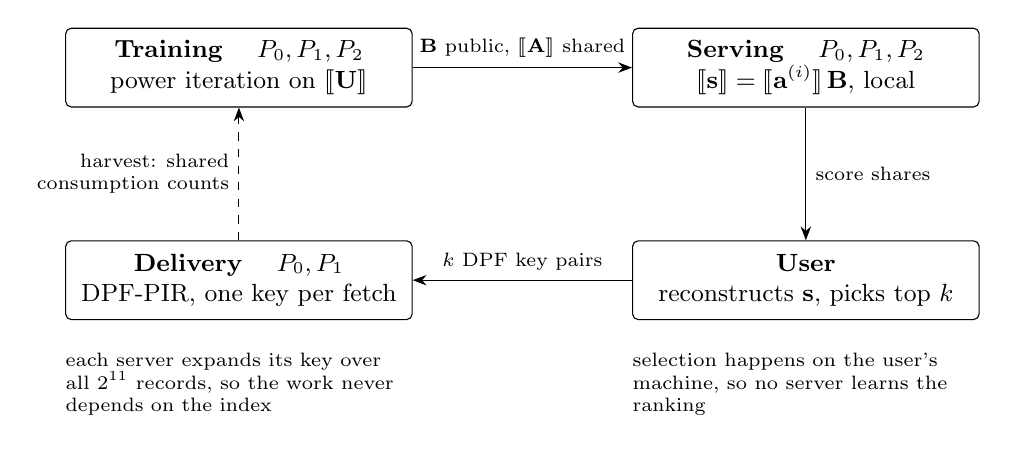
\begin{tikzpicture}[
    font=\small,
    box/.style={draw, rounded corners=2pt, align=center, inner sep=4pt,
                minimum height=10mm},
    note/.style={font=\scriptsize, align=left, text width=44mm},
    >={Stealth[length=5pt]}
  ]
  \node[box, minimum width=44mm] (train) at (0,0)
    {\textbf{Training} \quad $\party{0}, \party{1}, \party{2}$\\
     power iteration on $\shr{\ratings}$};
  \node[box, minimum width=44mm] (serve) at (7.2,0)
    {\textbf{Serving} \quad $\party{0}, \party{1}, \party{2}$\\
     $\shr{\mathbf{s}} = \shr{\avec{i}}\,\itemembed$, local};
  \node[box, minimum width=44mm] (user) at (7.2,-2.7)
    {\textbf{User}\\ reconstructs $\mathbf{s}$, picks top $\topk$};
  \node[box, minimum width=44mm] (pir) at (0,-2.7)
    {\textbf{Delivery} \quad $\party{0}, \party{1}$\\
     DPF-PIR, one key per fetch};

  \draw[->] (train) -- node[above, font=\scriptsize]{$\itemembed$ public,
    $\shr{\userembed}$ shared} (serve);
  \draw[->] (serve) -- node[right, font=\scriptsize]{score shares} (user);
  \draw[->] (user) -- node[above, font=\scriptsize]{$\topk$ DPF key pairs} (pir);
  \draw[->, dashed] (pir) -- node[left, font=\scriptsize, align=right]
    {harvest: shared\\ consumption counts} (train);

  \node[note, below=3mm of pir] {each server expands its key over all
    $2^{11}$ records, so the work never depends on the index};
  \node[note, below=3mm of user] {selection happens on the user's machine,
    so no server learns the ranking};
\end{tikzpicture}
\caption{The \sys{} cycle. Solid arrows run in every experiment in this report.
The dashed harvest arrow is implemented and tested as a library path
(Section~\ref{sec:design:harvest}) but is not yet driven by the networked server
binaries, and every training run here reads its ratings from disk.}
\label{fig:system}
\end{figure}

\subsection{Training}
\label{sec:design:train}

Training takes $\shr{\ratings}$ and runs \nudgeplain{}'s $\ApproxFactor$ under
replicated sharing: for each component, $\iters$ rounds of two shared
matrix--vector products, a projection against the rows of $\itemembed$ already
found, and a normalisation. Appendix~\ref{app:protocols} gives it as
Algorithm~\ref{alg:factor}. Three pieces of it need design decisions of their
own.

\paragraph{Where truncations go.} Ratings are integers, held at scale zero, so the
two matrix products need no truncation of their own, only a fixed rescaling
shift afterwards that keeps $\norm{\mathbf{v}}^2$ from overflowing. The remaining
truncations sit in orthogonalisation and normalisation, and each costs a
three-round protocol. Orthogonalisation can be \emph{deferred}: subtract the
projections at scale $3\fracbits$ and truncate once by $2\fracbits$. Or it can be
\emph{immediate}: truncate the inner products first and the result afterwards,
two truncations that never exceed scale $2\fracbits$. Deferral saves a
truncation and costs $\fracbits$ bits of headroom, and whether that fits depends
on $\bits$, $\fracbits$, $\items$ and $\dime$. So \sys{} derives the schedule from
public parameters at start-up, proves it fits with at least eight spare bits, and
refuses to run otherwise. At $\bits = 64$ on MovieLens-100K the deferred schedule
does not fit and training uses the immediate one, with 21 bits to spare. At
$\bits = 128$ the deferred schedule fits with 67.

\paragraph{How to normalise.} Normalising needs $1/\norm{\mathbf{v}}$ on a
shared $\mathbf{v}$. \sys{} has two implementations behind one interface. The
spec-faithful one follows \nudgeplain{}: a DCF-based gate finds the most
significant non-zero bit of $\norm{\mathbf{v}}^2$, which gives a first
approximation to $1/\norm{\mathbf{v}}$, and Newton--Raphson refines it. It
reveals nothing. The second opens $\norm{\mathbf{v}}^2$, divides in the clear,
and rescales by a public constant. It is far cheaper and it leaks, and
Section~\ref{sec:threat:gaps} states exactly what that costs the security
argument. Every result records which normaliser produced it.

\paragraph{Keeping $\itemembed$ public.} Because each finished row of
$\itemembed$ is opened, projecting against it is a product of shares with public
values, which needs no multiplication protocol. Our implementation priced the
alternative: keeping $\itemembed$ shared makes one small orthogonalisation cost
6 rounds and 1{,}800 bytes where the public version costs none. We keep
\nudgeplain{}'s choice, and Section~\ref{sec:leak} measures its consequence.

\subsection{Serving}
\label{sec:design:serve}

Each server holds a share of the user's embedding $\avec{i}$ and the public
$\itemembed$, so it computes its share of all $\items$ scores locally, with no
communication between servers. The user also supplies a shared mask carrying a
large negative sentinel at the items it has already rated. The servers add it to
their shares, which is again local, and send the result to the user, who
reconstructs the score vector and selects the top $\topk$.

The design draft specified an oblivious top-$\topk$ selector run by the servers.
We cut it: once the user reconstructs the scores, no server learns the selection
whether or not an oblivious selector exists, so the selector would protect
something already protected. The cost is that the user downloads a score share of
length $\items$ from each server, which Section~\ref{sec:limits} returns to.

\subsection{Delivery}
\label{sec:design:deliver}

Records are packed to a fixed width of $L = 256$ bytes, since a variable-width
record would leak its identity through the reply length. MovieLens-100K's 1{,}682
items pad to a domain of $2^{11} = 2{,}048$ entries, and padding records are all
zero, which leaks nothing because they are the same width as real ones. The DPF
is a two-party primitive, so $\party{0}$ and $\party{1}$ answer PIR queries and
$\party{2}$ does not. All three servers hold the catalogue, which is public. For
each of its $\topk$ recommendations the user sends one key to each PIR server,
and the difference of the two answers is the record.

\subsection{Closing the loop}
\label{sec:design:harvest}

When a PIR server expands a key, the expansion it computes is its share of the
indicator vector of the fetched item. \pirsonaplain{}'s observation is that this
is exactly a secret-shared record of consumption, already computed and normally
thrown away. \sys{}'s answer routine returns the expansion alongside the answer,
an accumulator sums it over queries, and a one-round conversion turns the two PIR
servers' 2-of-2 shares into the 2-of-3 replicated form training consumes. A
further one-round check, added after Section~\ref{sec:leak:malicious} found the
need for it, confirms that each query carries weight exactly one.
Algorithm~\ref{alg:harvest} gives both.

We state the extent of this plainly. The harvest, the conversion and the weight
check are implemented, and a test drives real PIR queries through them and
multiplies the result under the training substrate. The networked server
binaries do not yet accumulate expansions across sessions or retrain from them,
and every training run in this report reads MovieLens ratings from disk.

\subsection{Design decisions}
\label{sec:design:decisions}

Table~\ref{tab:decisions} collects the decisions that shape everything else,
each with the reason recorded when it was taken.

\begin{table}[t]
\centering
\small
\caption{The design decisions that matter most, from the project's decisions
log.}
\label{tab:decisions}
\begin{tabular}{@{}p{5.0cm} p{9.6cm}@{}}
\toprule
Decision & Reason \\
\midrule
Power iteration, not gradient descent & Matrix--vector products cost
  communication in the output length only, so only truncation and normalisation
  are expensive. This is \nudgeplain{}'s core idea. \\
Three servers, 2-of-3 replicated sharing, semi-honest & Matches \nudgeplain{}
  exactly, one fewer non-colluding party than \pirsonaplain{}'s four. \\
$\itemembed$ opened row by row & Makes orthogonalisation local. The cost is the
  leakage measured in Section~\ref{sec:leak}. \\
One DPF implementation for both halves & The same primitive is the PIR query and,
  through the DCF built beside it, the comparison gate. Forking it would double
  the code most likely to be wrong. \\
Top-$\topk$ on the user's machine & The user reconstructs the scores anyway, so a
  server-side oblivious selector would protect nothing further. \\
Fixed-width records & A variable width leaks the record through the reply
  length. \\
Ring width a template parameter & Whether $\bits = 64$ suffices was an open
  question, and the answer turned out to depend on which normaliser runs
  (Section~\ref{sec:eval:ring}). \\
Three OS processes, no threads & Each server serves one client to completion, so
  nothing is concurrent, and separate processes make that true rather than
  likely. \\
\bottomrule
\end{tabular}
\end{table}

%  5  Implementation
%% ==========================================================================
%%  FINAL REPORT --- SECTION 5, IMPLEMENTATION
%%  Sources: tech_dpf.tex, tech_serving.tex and tech_net.tex (the mid-term
%%  technical report, rewritten here because it predates private training and
%%  says so throughout), the headers under include/oblivrec/, and the output
%%  of `mingw32-make test`, which prints every number quoted below that is not
%%  from bench/results/.
%% ==========================================================================
\section{Implementation}
\label{sec:impl}

\sys{} is written in C++17 with no cryptographic library. It comprises about
7{,}400 lines of library and application code and about 3{,}300 lines of tests
in eighteen test binaries, with Python for the cleartext oracle, the export of
fixed-point models and the leakage studies. The pseudorandom generator is fixed-key
AES-128 in Davies--Meyer mode through AES-NI instructions, and key material comes
from the operating system's generator. Table~\ref{tab:layout} maps the code. The
repository also vendors \nudgeplain{}'s Go reference implementation under
\texttt{third\_party/}, under its MIT licence, as a reference to read alongside the
paper. No build target compiles or links it.

\begin{table}[t]
\centering
\small
\caption{Where each part of the system lives.}
\label{tab:layout}
\begin{tabular}{@{}l p{11.2cm}@{}}
\toprule
Directory & Contents \\
\midrule
\texttt{src/dpf/} & The DPF: tree generation, single-point and whole-domain
  evaluation, key serialisation, and the DCF built beside it. \\
\texttt{src/mpc/} & Replicated sharing, pairwise-PRF zero shares, shared
  matrix--vector products, truncation, the MSNZB comparison gate and the
  shared inverse square root. \\
\texttt{src/mf/} & Power iteration under sharing, orthogonalisation, both
  normalisers, the truncation schedule, and a cleartext fixed-point twin. \\
\texttt{src/serve/}, \texttt{src/pir/} & Score shares and the seen-item mask.
  The catalogue, the PIR server and client, and the harvest. \\
\texttt{src/net/} & Length-prefixed TCP framing, the transcript recorder, and
  channel-level network emulation. \\
\texttt{src/apps/} & The three servers, the training driver, the end-to-end
  demo, and the probe used by the distinguisher. \\
\texttt{model/} & The cleartext oracle, the float-to-ring export, the
  reconstruction attack, and the differential-privacy and poisoning studies. \\
\texttt{bench/} & Seven benchmarks writing one JSON row per measurement, and the
  script that draws every figure from those rows. \\
\bottomrule
\end{tabular}
\end{table}

\subsection{The distributed point function}
\label{sec:impl:dpf}

The DPF follows Boyle, Gilboa and Ishai~\cite{bgi2016}. It is written by us
rather than imported because it is the component both halves depend on, and a
viva will probe it hardest.

\paragraph{Key size.} A key holds a header, an initial seed, one correction word
of 18 bytes per level, and a final correction word of $\lceil \bits/8 \rceil$
bytes, so its size is $1 + 4 + 16 + 18D + \lceil \bits/8 \rceil$ bytes for a
domain of $D$ bits. The serialiser's reported size is asserted equal to the
length it actually writes. At the 11 domain bits MovieLens-100K needs, a key is
227 bytes against 16{,}384 bytes for a naive one-hot query, and the gap widens
without bound (Figure~\ref{fig:keysize}). Measuring it corrected the design
draft, which had estimated 260 bytes at 4{,}096 items. The measured value is 245
bytes, and the draft's formula had omitted the seed and the header while
evaluating at the wrong domain width.

\begin{figure}[t]
\centering
\includegraphics[width=0.62\linewidth]{fig_keysize}
\caption{Query size against catalogue size. The DPF key grows by 18 bytes per
domain bit while the naive query doubles. The star is the operating point of every
experiment in this report. The plotted closed form is the one
\texttt{tests/test\_dpf\_serialize.cpp} asserts equal to the serialised length.
Generated by \texttt{mingw32-make figures}.}
\label{fig:keysize}
\end{figure}

\paragraph{Sign convention.} Textbook presentations negate party one's output,
which gives the sum $\Eval(k_0, x) + \Eval(k_1, x) = f(x)$. Our specification
states the invariant as a difference, so we omit the negation and have
$\Eval(k_0, x) - \Eval(k_1, x) = f(x)$ at every interface, in the PIR read and in
the harvest. The DCF uses the textbook convention internally, as its construction
is defined, and converts at its boundary. Getting the convention backwards makes
every test fail in a way that looks like a traversal bug rather than a sign
error, so it is recorded at every use.

\paragraph{Key material.} The two initial seeds are the entire secret. The first
version seeded them from a Mersenne Twister, which is a genuine break: that
generator is reconstructible from 624 consecutive outputs, so an adversary who
saw enough key material could rebuild the tree and recover $\alpha$. Seeds now
come from the operating system's generator, and the failure policy is to abort
rather than fall back to a weaker source.

\paragraph{Exhaustive verification.} The characteristic failure of this
construction is a wrong control-bit update, which stays invisible until enough
levels accumulate and then presents as ``correct at two domain bits, wrong at
eight''. So the tests walk both parties' trees in lockstep and assert the
structural invariant at every internal node: on the path to $\alpha$ the seeds
differ and the control bits disagree, and off it both are equal. The difference
invariant itself was then checked for every $\alpha$ against every $x$ in every
domain up to 16 bits on the 64-bit ring and 15 bits on the 128-bit ring, which is
$7.16 \times 10^9$ leaf comparisons. That sweep passed at commit
\texttt{bce4cb1}. The default test target repeats it up to 11 bits on both rings
in about a second, and $\beta$ is derived from the domain and $\alpha$ so that
billions of comparisons do not all exercise the final correction word at one
value.

\paragraph{A bug found by testing the wire format.} Deserialisation accepted a
party byte outside $\{0, 1\}$. Evaluation starts its control bit at the party
index and branches on whether it is non-zero, so a party byte of 7 made the key
\emph{silently evaluate as party one}. Keys arrive over the network, so the party
byte and the domain width are now validated before either is used, and the tests
that found the bug are kept as regression tests.

\subsection{Private serving and delivery}
\label{sec:impl:serve}

\paragraph{The catalogue.} MovieLens-100K's item file is variable-length text, so
each record is packed into 256 bytes with explicit one-byte length prefixes
rather than delimiters. The file contains Latin-1 bytes and does not decode as
UTF-8, so it is read and carried as raw bytes. The longest record uses 117 bytes,
and every record is checked against the budget at load time, so a longer title
fails loudly at start-up rather than being cut at answer time.

\paragraph{The read.} Each PIR server expands its key over all 2{,}048 indices
and takes an inner product with the catalogue, viewed as 32 ring words per
record at $\bits = 64$. Two properties carry the obliviousness claim. The loop
visits every record in index order with no branch on the data, and every expanded
coefficient is a pseudorandom share, so there is no sparse pattern for a
compiler, a cache or a timing observer to find. Reads are checked byte for byte
against a cleartext lookup at 60 random indices on the 64-bit ring and 20 on the
128-bit ring, including both ends of the domain and padding slots.

\paragraph{Scores.} Both factors of a score are encoded at $\fracbits = 20$
fractional bits, so scores are at scale $2\fracbits$, and serving decodes at that
scale instead of truncating, because truncation is interactive. Getting this
wrong would scale every score by $2^{20}$, which is monotone and therefore
invisible in a ranking, so it is recorded explicitly. The seen-item sentinel is
$-2^{55}$, about $3{,}700\times$ below the largest real score and $256\times$
above the bottom of the ring, both asserted. The top-$\topk$ comparison is signed,
because comparing two's-complement values as unsigned would sort the masked items
first.

\paragraph{The float-to-ring boundary.} One program converts floats to ring
elements, and a committed file of 25 value pairs checks it against the C++ side
on every test run. It found two bugs on its first run. Python's \texttt{rint}
rounds half to even while C++'s \texttt{round} rounds half away from zero, so the
two disagreed at every exact half-quantum. And the reference scores had been
computed by quantising the float product, while the protocol multiplies quantised
factors, so the two disagreed on 1{,}650 of 1{,}682 scores by about $5 \times
10^{-6}$ relative. That is irrelevant to the ranking, which is exactly why a
tolerance-based check would have accepted it. Serving is now checked against the
oracle by exact equality, and all 1{,}682 scores match.

\paragraph{Three processes.} The servers are three operating-system processes
that exchange length-prefixed frames over TCP. TCP is a byte stream, so one
\texttt{send} can arrive as several \texttt{recv} calls. The test forces this with
a deliberately small receive buffer and checks that a 16{,}384-byte frame arrives
as one frame. The declared frame length is attacker-chosen and is checked against
a cap before it sizes any allocation. Every frame can be recorded at the channel
boundary into a transcript, which Section~\ref{sec:eval:wire} analyses.

\subsection{The training substrate}
\label{sec:impl:mpc}

\paragraph{Sharing and zero shares.} \texttt{Mpc3} holds all three parties' state
and moves every inter-party message through one exchange routine, which counts
rounds and bytes. That counter is what every cost in Section~\ref{sec:eval} is
read from, so a protocol cannot send without paying. Zero shares come from three
pairwise PRF generators.

\paragraph{The counter invariant.} The three generators must advance in lockstep.
A protocol that draws masks for only two of the three parties leaves the third
generator one step behind, and every later zero share then fails to sum to zero.
Nothing crashes: the parties go on producing well-formed shares of the wrong
value. This happened once and silently corrupted every subsequent multiplication.
The exchange routine now asserts that all three counters agree, and protocols in
which one party draws nothing advance its generator explicitly.

\paragraph{Theorem~4.2, asserted.} The tests check \nudgeplain{}'s central cost
claim against the byte counter rather than in prose: multiplying a shared
$4 \times 64$ matrix by a shared vector costs one round and 96 bytes, which is
three parties sending four 8-byte elements each, set by the four outputs and not
by the 256 matrix entries.

\subsection{Truncation}
\label{sec:impl:trunc}

\texttt{TruncatePair} is the standard correct construction. A helper party draws
$r$ and gives the other two parties shares of $r$ and of $r \gg \fracbits$. Those
two open $x - r$ between themselves, shift it in the clear, add back their shares
of $r \gg \fracbits$, and reshare under a pairwise mask the helper cannot
compute (Algorithm~\ref{alg:trunc}). It costs three rounds and eight ring elements
per value. Over 3{,}200 random values its error is
never more than one unit in the last place. The naive alternative, where every
party shifts its own shares, costs nothing and is catastrophically wrong on about
a quarter of values in our tests, because the shares wrap the ring. That
comparison is the whole argument for paying three rounds, and
Section~\ref{sec:eval:stages} shows the three rounds are most of what training
costs. The helper is a parameter at every call site, because a helper that also
saw the opening would learn $x$.

\subsection{The comparison gate and the normaliser}
\label{sec:impl:norm}

\paragraph{The DCF.} The design draft had asserted that a DPF and a DCF are the
same primitive. They are not, and \nudgeplain{}'s reference implementation keeps
them in separate modules. A DCF is non-zero on a whole prefix of the domain, so
every node of its tree carries a value word as well as a seed, and every level
needs a value correction word that depends on everything below it. We built it
beside the DPF, sharing the pseudorandom generator, and verified it the same
way: every threshold against every input, exhaustively up to 7 domain bits on the
64-bit ring and 6 on the 128-bit ring.

\paragraph{The MSNZB gate.} The normaliser needs the most significant non-zero
bit of a shared value $S = \norm{\mathbf{v}}^2$. The gate uses the
mask-and-reveal technique of Section~\ref{sec:background:fss}. Offline, a dealer
draws $r$ and builds one DCF key pair per threshold $2^k$, shifted by $r$. Online,
the parties open $c = S + r$ and evaluate every key at $c$. Since
$\sum_k 1[S \ge 2^k]$ counts the thresholds below $S$, any step function of
$\mathrm{msnzb}(S)$ is a public linear combination of those indicators. The seed
for $1/\norm{\mathbf{v}}$, a power of two within a factor of $\sqrt{2}$ of it, is
one such function. All
thresholds share one opening, so the gate costs two rounds, one to open and one to
reshare, however many thresholds it covers. Algorithm~\ref{alg:msnzb} gives the
gate and the Newton iteration it seeds.

\paragraph{Why the gate needs a 128-bit ring.} The opening $c = S + r$ hides $S$
only if $r$ comes from a range $\kappa$ bits wider than $S$'s. With $\kappa = 40$
and the values power iteration produces, the DCF domain needs 81 bits. A 64-bit
ring has no room for the mask at all, so \texttt{FssNormalizer} refuses to
construct at $\bits = 64$ rather than masking with too few bits, since a gate that
did so would look like privacy while providing none.

\paragraph{Inverse square root.} \texttt{InvSqrtShared} takes the gate's seed and
refines it with Newton--Raphson. Four steps reach a worst relative error of $1.41
\times 10^{-6}$ over our test values, for 50 rounds in total. The step count was
chosen from a cleartext reference first, which measured the error at every step
count before any shared code existed.

\paragraph{The gate cannot check its own range.} The gate covers thresholds from
$2^{\mathit{lo}}$ to $2^{\mathit{hi}}$. A value outside that range does not raise
an error. It clamps, because the answer is a telescoping sum over the thresholds.
And the gate cannot check, because it only ever sees $S + r$, and learning
$\mathrm{msnzb}(S)$ is precisely what it exists to avoid. So the caller must size
the range from public parameters. Section~\ref{sec:impl:bugs} describes what
happened when a caller did not.

\subsection{Power iteration}
\label{sec:impl:factor}

\texttt{ApproxFactorShared} runs Algorithm~\ref{alg:factor} with the truncation
schedule and either normaliser. On a small test instance it agrees with its
cleartext fixed-point twin to $1.5 \times 10^{-6}$ in $1 - \abs{\cos}$ per row,
with every row of $\itemembed$ unit length to $3.2 \times 10^{-6}$. The
start-up headroom assertion is not decorative. It refuses $\fracbits = 30$ at
$\bits = 64$, and it caught a real overflow: $\norm{\mathbf{v}}^2$ of a vector
not yet normalised needs 84 bits, which led to the fixed rescaling shift applied
right after the two matrix products.

The training driver writes $\itemembed$ and shares of $\userembed$ to disk, and
the demo serves them. \texttt{demo} with the privately trained, spec-faithful
model at $\bits = 128$ returns ten film titles for user 42, headed by
\emph{Toy Story}. Each record is byte-exact against a cleartext lookup, and the
ranking agrees position for position with an independently computed reference.
That run is the composition end to end: a model no server saw in the clear,
served from shares, delivered without either PIR server learning what was
fetched.

\subsection{Bugs found by measurement}
\label{sec:impl:bugs}

The project's rule was that every private component is checked against a
cleartext twin, and every approximate protocol has its error measured rather than
assumed. Table~\ref{tab:bugs} lists what that found. None of these would have
been found by reading the code, and most produced no error at all.

\begin{table}[t]
\centering
\small
\caption{Defects found by tests and measurements rather than by inspection.}
\label{tab:bugs}
\begin{tabular}{@{}p{4.3cm} p{4.4cm} p{5.8cm}@{}}
\toprule
Defect & How it was found & What it would have caused \\
\midrule
DPF party byte unvalidated & serialisation tests & a malformed key silently
  evaluates as the other party \\
Rounding mode differs across the Python and C++ boundary & 25-vector contract
  test & off-by-one ring elements at every half-quantum \\
Reference quantised the product, protocol the factors & exact score comparison &
  1{,}650 of 1{,}682 scores wrong, invisible to a tolerance check \\
PRF counters out of step & multiplication tests & well-formed shares of the wrong
  value, every product after the first \\
$\norm{\mathbf{v}}^2$ overflows before normalisation & start-up headroom
  assertion & silent wrap of the ring, a meaningless model \\
MSNZB gate range too narrow & quality study on the no-leak path & 0.108 of
  nDCG@20 lost at $\iters = 10$, with identical cost \\
Transcript writers interleaved & parsing the transcript & invalid JSON in the
  evidence file \\
\bottomrule
\end{tabular}
\end{table}

The gate-range bug deserves its own paragraph, because it is the one that nearly
became a finding. The training driver first called the MSNZB gate with the range
$[\fracbits - 8, \fracbits + 8]$, copied from the parameter sweep. Values outside
it clamped, Newton--Raphson started from the wrong power of two, and the power
iteration never converged: it ended orthogonal to the oracle's subspace. At
$\iters = 10$ the no-leak model scored 0.3428 against 0.4513 for the revealing
path, which would have been reported as ``revealing nothing costs 24\% of
recommendation quality''. The range is now $[1, 2\fracbits + 8]$ and the gap is
0.0020. Rounds and bytes are \emph{identical} under both ranges, because a wider
range buys more DCF keys offline while the online gate stays two rounds, which is
why the cost benchmark that first used the gate could never have caught it. The
rows from the buggy run were not kept, so the two nDCG values above are recorded
in the commit that fixed it (\texttt{d2138ad}) and in the comment at the gate's
call site, not in the committed data.

%  6  Evaluation   (F3 F4 F5 F7 F8 F9 F12)
%% ==========================================================================
%%  FINAL REPORT --- SECTION 6, EVALUATION
%%  Every number below is recomputable from the newest-sha rows of the named
%%  bench/results/*.jsonl file, the same filter make_figures.py applies.
%%  Figures F3 F4 F5 F7 F8 F9 F12 live here, each exactly once.
%% ==========================================================================
\section{Evaluation}
\label{sec:eval}

This section asks what private training and private delivery each cost, what
they cost together, where the cost goes, and what it does to recommendation
quality. It reports two results that go against the system in the body rather
than in a footnote.

\subsection{Setup}
\label{sec:eval:setup}

All measurements use MovieLens-100K's \texttt{u1} split (943 users, 1{,}682
items, 80{,}000 training ratings) at $\dime = 16$, $\iters = 10$ and $\fracbits =
20$, with $\bits = 64$ and the revealing normaliser unless stated. Delivery
fetches $\topk = 10$ records per session, and quality is nDCG@20. The machine is
a Windows~11 laptop, and the code is built by MSYS2's g++.

\paragraph{Network profiles.} We use four: \texttt{local}, \texttt{lan} (1\,ms
round trip, 1\,Gbit/s), \texttt{wan\_a} (30\,ms, 100\,Mbit/s) and \texttt{wan\_b}
(100\,ms, 10\,Mbit/s). The development machine has neither Docker nor kernel
network emulation, so the profiles are applied at the channel level. Delivery
runs over real sockets wrapped in a channel that delays each frame. Training runs
its three parties in one process, so its time on a profile is computed from the
exactly counted rounds and bytes as rounds times round-trip time plus bytes over
bandwidth. We call this channel-level emulation throughout and never kernel
emulation.

\paragraph{What to trust.} Round and byte counts are exact and deterministic.
Absolute timings on this laptop vary by up to a factor of four between
back-to-back runs, while repetitions within one run agree closely, which is the
pattern of thermal throttling. So we quote ratios taken within one run, and where
a number derived from absolute times moves between runs we give the range we
observed. Every figure is drawn by \texttt{mingw32-make figures} from the newest
commit's rows in the named data file, and Appendix~\ref{app:reproduce} maps each
one to the command that produces it.

\subsection{Recommendation quality}
\label{sec:eval:quality}

Table~\ref{tab:quality} compares private training with the cleartext oracle, which
runs the same power iteration in floating point. The revealing path at
$\bits = 64$ stays within 0.007 of the oracle at every $\iters$. Fixed-point
arithmetic and a real truncation protocol cost essentially nothing in quality.

\begin{table}[t]
\centering
\small
\caption{nDCG@20 against the number of power iterations $\iters$, at $\dime = 16$.
The $\bits = 128$ revealing column is the control that isolates the normaliser:
it shares the spec-faithful path's ring and truncation schedule and differs only
in revealing the norm. The last column is the no-leak path's loss against that
control. Data: \texttt{bench/results/train\_quality.jsonl}.}
\label{tab:quality}
\begin{tabular}{@{}rccccc@{}}
\toprule
$\iters$ & reveal, $\bits = 64$ & reveal, $\bits = 128$ & \textbf{no leak},
  $\bits = 128$ & oracle & no-leak cost \\
\midrule
1  & 0.3729 & 0.3727 & \textbf{0.1651} & 0.3664 & 0.2076 \\
2  & 0.4251 & 0.4248 & 0.4230 & 0.4220 & 0.0019 \\
5  & 0.4485 & 0.4490 & 0.4448 & 0.4455 & 0.0041 \\
10 & 0.4511 & 0.4513 & 0.4493 & 0.4536 & 0.0020 \\
25 & 0.4532 & 0.4531 & 0.4499 & 0.4545 & 0.0031 \\
50 & 0.4531 & 0.4532 & 0.4502 & 0.4525 & 0.0030 \\
\bottomrule
\end{tabular}
\end{table}

\paragraph{Revealing nothing costs little quality.} For every $\iters \ge 2$ the
spec-faithful normaliser loses between 0.0018 and 0.0041 of nDCG@20 against
either revealing column. The $\bits = 128$ revealing column is what makes that
claim defensible. Without it, the comparison would confound the normaliser with
the ring width and the deferred truncation schedule that $\bits = 128$ allows.
The two revealing columns differ by at most 0.0005, so the normaliser accounts
for the whole gap. What revealing nothing costs instead is rounds: 11{,}519
against 2{,}191 at $\iters = 10$ and $\bits = 128$, a factor of 5.3.

\paragraph{The exception at $\iters = 1$.} With a single power iteration the
no-leak path scores 0.1651 against 0.3729. The first normalisation acts on the
raw random start vector, and a single iteration leaves nothing downstream to
recover from whatever error it introduces. We have not isolated the mechanism
further. From $\iters = 2$ the gap closes. Nobody would choose $\iters = 1$, but
the cliff is sharp and we report it.

\paragraph{Quality is flat in $\iters$.} The oracle's own sweep settles how many
iterations are worth paying for (Figure~\ref{fig:ell}). Across a fortyfold
increase in $\iters$ the subspace angle to the true singular subspace falls by
five orders of magnitude, from 0.97 radians to $6.7 \times 10^{-6}$, while
nDCG@20 stays between 0.4523 and 0.4545. Ranking needs a subspace good enough to
order the scores stably, not the singular vectors themselves. The slow
convergence has a visible cause: the sixteenth and seventeenth squared singular
values differ by only 3\%. Since rounds grow linearly in $\iters$
(Section~\ref{sec:eval:sweep}), this flatness is what makes $\iters = 10$ the
right operating point.

\begin{figure}[t]
\centering
\includegraphics[width=0.62\linewidth]{fig_ell}
\caption{The cleartext oracle at $\iters$ from 10 to 400. nDCG@20 spans 0.002
while the subspace angle spans five orders of magnitude. Data:
\texttt{bench/results/oracle\_ell\_sweep.jsonl}.}
\label{fig:ell}
\end{figure}

\subsection{The cost of each half, isolated}
\label{sec:eval:compose}

The central comparison runs five arms in one process, interleaved repetition by
repetition so that thermal drift cannot line up with arm identity
(Table~\ref{tab:compose} and Figure~\ref{fig:compose}). B1 trains in the clear
and fetches in the clear. B2 swaps in DPF-PIR. B3 swaps in private training
instead. FULL is \sys{}. B5 trains in the clear and downloads the whole catalogue.
Training is amortised over the 943 users one training run serves.

\begin{table}[t]
\centering
\small
\caption{Per-session cost of each arm, with training amortised over 943 users.
Bytes and rounds are exact. Times are channel-level emulation. Data:
\texttt{bench/results/bench\_compose.jsonl}.}
\label{tab:compose}
\begin{tabular}{@{}llrrrrc@{}}
\toprule
Arm & training, delivery & bytes & rounds & \texttt{local} (ms) &
  \texttt{wan\_a} (ms) & nDCG@20 \\
\midrule
B1   & clear, clear         & 2{,}600   & 10 & 1.19 & 301.4 & 0.454 \\
B2   & clear, DPF-PIR       & 9{,}660   & 10 & 3.11 & 303.9 & 0.454 \\
B3   & private, clear       & 71{,}264  & 13 & 2.02 & 397.7 & 0.451 \\
FULL & private, DPF-PIR     & 78{,}324  & 13 & 3.96 & 400.2 & 0.451 \\
B5   & clear, full download & 430{,}592 & 1  & 1.16 & 65.6  & 0.454 \\
\bottomrule
\end{tabular}
\end{table}

\paragraph{Composing costs exactly the sum of the halves.} $\mathrm{FULL} =
\mathrm{B2} + \mathrm{B3} - \mathrm{B1}$ holds to the byte. Over a whole training
run plus one session it is 64{,}760{,}124 bytes, and the benchmark asserts the
identity before it writes a single row, so a regression that broke additivity
could not produce a figure. On \texttt{wan\_a}, private delivery adds 2.5\,ms per
session and private training adds 96\,ms, and quality moves from 0.454 to 0.451.

\paragraph{The result that goes against us.} On \texttt{wan\_a}, B5 is 4.6 times
\emph{faster} than B2, although it sends 45 times as many bytes. Delivery as
built costs one round trip per recommendation, ten in all, while B5 pays one. At
30\,ms per trip, round trips decide the outcome and bytes barely matter.
Sending all ten key pairs in one round trip reverses it: the model puts batched
B2 at 33.9\,ms against B5's 65.6\,ms. We did not implement batching, and the
benchmark marks those rows as not implemented. The honest summary is that
private delivery as built is cheap in bytes and expensive in round trips, and the
fix is known and unbuilt.

\begin{figure}[t]
\centering
\includegraphics[width=\linewidth]{fig_compose}
\caption{Left: what each arm adds over B1, per session, on \texttt{local} and
\texttt{wan\_a}. Right: the \texttt{wan\_a} session time as built, against the
modelled time with the $\topk$ queries batched into one round trip, which is not
implemented. Data: \texttt{bench/results/bench\_compose.jsonl}.}
\label{fig:compose}
\end{figure}

\subsection{The private read against its alternatives}
\label{sec:eval:pir}

Figure~\ref{fig:pircost} compares one private read with a cleartext lookup (B1)
and with downloading the whole catalogue (B5), the first alternative a reader
proposes because 430\,KB does not sound large. DPF-PIR sends 483 bytes to each
server, so it moves 446 times fewer bytes than B5 counting both servers. It is
also the slowest of the three in server CPU, about five times slower than B5's
local copy in both committed runs (5.3 and 5.6), and four orders of magnitude
slower than a cleartext lookup. Its advantage is entirely in communication.

Setting the extra server time against the saved bytes gives the link speed below
which the private read wins. That crossover is derived from absolute times, so it
moves with the machine's thermal state: 8.0\,Gbit/s in one committed run and
22.9\,Gbit/s in the run the figure shows. Either way it is far above any
wide-area link, and we would rather state the crossover than imply there is none.

\begin{figure}[t]
\centering
\includegraphics[width=0.9\linewidth]{fig_pir_cost}
\caption{One read at the MovieLens-100K operating point: 1{,}682 records of
256\,B in an 11-bit domain. Bytes are per server. Both panels must be read
together, since the left alone would be advocacy. Data:
\texttt{bench/results/bench\_baseline.jsonl}.}
\label{fig:pircost}
\end{figure}

\subsection{Scaling, and Theorem~4.2 measured}
\label{sec:eval:sweep}

The sweep varies one parameter at a time around the baseline, five repetitions
each, on all four profiles (Figure~\ref{fig:sweep}). It is not the Cartesian
product, so interactions between parameters are not measured.

\paragraph{Rounds.} Rounds are linear in $\dime$ (1{,}310, 2{,}686 and 5{,}438
at $\dime = 8, 16, 32$) and in $\iters$ (436 at $\iters = 1$, 6{,}436 at
$\iters = 25$), and flat in $\users$: 2{,}686 at 235, 471 and 943 users.

\paragraph{Bytes.} This is \nudgeplain{}'s Theorem~4.2 measured rather than
quoted. Quadrupling the input matrix, from 235 to 943 users, moves traffic from
62.03 to 64.75\,MB, an increase of 4.4\%. The increase is exactly linear at
3{,}840 bytes per added user, which is the one term in the cost that depends on
$\users$: each of the $\dime\iters = 160$ iterations computes
$\ratings\mathbf{v}$, an $\users$-vector, and resharing it costs three parties
one 8-byte element per entry, so $160 \times 3 \times 8 = 3{,}840$ bytes per
user. Communication tracks the largest intermediate vector, not the input matrix.

\paragraph{Training is round-bound.} On \texttt{wan\_a} one training run takes
85.8\,s, of which 80.6\,s is round-trip latency and 5.2\,s is transfer. Anything
that removes rounds matters far more than anything that removes bytes, which is
why the next subsection counts rounds.

\begin{figure}[t]
\centering
\includegraphics[width=\linewidth]{fig_sweep}
\caption{Left: rounds against $\dime$, $\iters$ and $\users$. Right: traffic
against the size of the input matrix. The matrix grows fourfold and traffic by
4.4\%. Data: \texttt{bench/results/bench\_sweep.jsonl}.}
\label{fig:sweep}
\end{figure}

\subsection{Where the rounds go}
\label{sec:eval:stages}

Table~\ref{tab:stages} attributes every round and byte of one training run to
the stage that spent it, in the three configurations. The attribution is a closed
form derived from each protocol's structure, then validated against a real run:
the residual is zero rounds and zero bytes in all three configurations, and the
benchmark exits with an error if it is not. So these are shares of a complete
budget, not a sample. A zero residual alone would not catch rounds attributed to
the wrong stage, so a second, independent count checks that too. A wrapper around
the normaliser meters every round spent inside it, and the model must predict
that count exactly, including the truncations the normaliser makes internally.
It does in all three configurations: 880 rounds for each revealing path and
10{,}208 for the path that reveals nothing.

\begin{table}[t]
\centering
\small
\caption{Rounds per training run by stage, with each stage's share of rounds and
of bytes. ``Open $\itemembed$'' is the sixteen row openings. Data:
\texttt{bench/results/bench\_stages.jsonl}.}
\label{tab:stages}
\begin{tabular}{@{}lrrrrrr@{}}
\toprule
 & \multicolumn{2}{c}{reveal, $\bits = 64$} & \multicolumn{2}{c}{reveal,
 $\bits = 128$} & \multicolumn{2}{c}{no leak, $\bits = 128$} \\
\cmidrule(lr){2-3}\cmidrule(lr){4-5}\cmidrule(l){6-7}
Stage & rounds & \% rounds / bytes & rounds & \% rounds / bytes & rounds &
  \% rounds / bytes \\
\midrule
matrix--vector & 320 & 11.9 / 15.6 & 320 & 14.6 / 15.6 & 320 & 2.8 / 14.0 \\
truncation & 1{,}998 & \textbf{74.4} / \textbf{83.4} & 1{,}503 & \textbf{68.6} /
  \textbf{83.4} & 8{,}367 & \textbf{72.6} / \textbf{75.1} \\
normalisation & 352 & 13.1 / 0.0 & 352 & 16.1 / 0.0 & 2{,}464 & 21.4 / 9.9 \\
FSS gate & 0 & 0 / 0 & 0 & 0 / 0 & 352 & 3.1 / 0.0 \\
open $\itemembed$ & 16 & 0.6 / 1.0 & 16 & 0.7 / 1.0 & 16 & 0.1 / 0.9 \\
\midrule
total & 2{,}686 & & 2{,}191 & & 11{,}519 & \\
\bottomrule
\end{tabular}
\end{table}

\paragraph{Truncation dominates, in every configuration.} It is 68.6 to 74.4\%
of rounds and 75.1 to 83.4\% of bytes. The FSS comparison gate, in the one
configuration that has it, is 3.1\% of rounds. The shared matrix--vector products
cost 320 rounds, one per product, and between 2.8 and 14.6\% of rounds.
Anyone optimising this system should start with truncation, whose three rounds
recur after every rescaling, every orthogonalisation and every Newton step. The
gate, which looks like the exotic part, is not the problem.

\paragraph{CPU ranks the stages differently.} Figure~\ref{fig:stages} also times
each operation on its own. The shared matrix--vector product over the full rating
matrix is the most expensive operation in CPU by a wide margin, while being cheap
in rounds. On a wide-area link the round count governs, and locally the CPU time
does, so which stage matters depends on where the servers are.

\begin{figure}[t]
\centering
\includegraphics[width=\linewidth]{fig_stages}
\caption{Left: each stage's share of the rounds in one training run, per
configuration. Right: median CPU time per call, each operation timed on its own.
Data: \texttt{bench/results/bench\_stages.jsonl}.}
\label{fig:stages}
\end{figure}

\subsection{How wide the ring must be}
\label{sec:eval:ring}

Whether a 64-bit ring suffices at MovieLens scale, or \nudgeplain{}'s 128 bits are
needed, was an open question in our design. It has two answers, for two different
reasons, and the tighter one wins.

\paragraph{Arithmetic headroom.} The truncation schedule is derived from public
parameters, and deriving it at larger scales answers the question without running
them. At $\fracbits = 20$ and $\bits = 64$, the deferred schedule does not fit at
any of the three scales we evaluated, MovieLens-100K, MovieLens-1M and a
Netflix-sized matrix, so training truncates immediately, with 21, 18 and 11 bits
to spare. At $\fracbits = 24$ and Netflix size there is no safe schedule at all.
At $\bits = 128$ the deferred schedule fits everywhere with at least 55 spare
bits, and at MovieLens-100K it needs fewer rounds (2{,}191 against 2{,}686) for
twice the bytes (129.3\,MB against 64.75\,MB).

\paragraph{The mask.} The spec-faithful normaliser's gate needs an 81-bit domain
to hide its input (Section~\ref{sec:impl:norm}). So a 64-bit ring is enough
arithmetically at MovieLens-1M, and not enough at any scale for a normaliser that
reveals nothing. That second constraint is not arithmetic, and it is the one that
decides the ring width.

\subsection{On the wire}
\label{sec:eval:wire}

An argument that message sizes do not depend on the fetched index, and a
measurement that they do not, are different claims. We recorded every frame at
the channel boundary while a probe issued 1{,}800 queries across three record
indices, 0, 777 and 1234, generating fresh keys for every query. Every query frame
is 228 bytes and every reply is 265 bytes, whatever the index.

We then trained a logistic-regression classifier on the raw frame bytes to tell
each pair of indices apart and scored it on 480 held-out queries per pair
(Table~\ref{tab:distinguisher} and Figure~\ref{fig:distinguisher}). Chance lies
inside every 95\% interval. The same pipeline run on deliberately shuffled labels
agrees with the real runs, which shows the harness measures what it claims to.

\begin{table}[t]
\centering
\small
\caption{Telling fetched indices apart from the wire bytes alone, with 480
held-out queries per pair and the same pipeline run on shuffled labels as a
control. Data: \texttt{bench/results/distinguisher\_result.jsonl}.}
\label{tab:distinguisher}
\begin{tabular}{@{}lcc@{}}
\toprule
Adversary & accuracy & 95\% interval \\
\midrule
index 0 against 1234   & 0.490 & 0.445 to 0.534 \\
index 0 against 777    & 0.494 & 0.449 to 0.538 \\
index 1234 against 777 & 0.500 & 0.455 to 0.545 \\
\midrule
shuffled labels        & 0.483 & 0.439 to 0.528 \\
\bottomrule
\end{tabular}
\end{table}

\begin{figure}[t]
\centering
\includegraphics[width=0.62\linewidth]{fig_distinguisher}
\caption{The distinguisher at chance. What matters is that 0.5 lies inside
every interval, not that the points sit near it. Data:
\texttt{bench/results/distinguisher\_result.jsonl}.}
\label{fig:distinguisher}
\end{figure}

This is not a proof. It says that one adversary, with one feature representation,
did not beat chance on this data. What it rules out is the failure that actually
occurs in practice, a length or byte pattern that correlates with the query.

\subsection{Server-side timing}
\label{sec:eval:timing}

Frame sizes are fixed, but a server whose running time depended on the index
would leak it to anyone who can time the reply. We timed the PIR answer routine
200 times at each of eight indices spread across the domain, interleaved rather
than in blocks so that thermal drift could not line up with the index
(Figure~\ref{fig:timing}). The mean call takes 87\,$\mu$s. The spread between
the eight per-index means is 1.7\,$\mu$s, smaller than the median standard
deviation of 6.0\,$\mu$s within a single index, and a permutation test on
shuffled index labels puts the observed spread at $p = 0.60$, in the middle of
the null distribution.

This is a bound, not a proof of constant time, because no finite sample shows a
difference is exactly zero. What it shows is that any index-dependent signal is
below 2.0\% of the mean call at this sample size. That is consistent with the
construction, which expands every node and takes an unconditional inner product
over every record. Timing on the wire itself is dominated by the operating
system's scheduler and network stack, and we did not analyse it.

\begin{figure}[t]
\centering
\includegraphics[width=\linewidth]{fig_timing}
\caption{Left: server time per call at eight record indices. Right: the spread
between index means, against its distribution under shuffled labels. Data:
\texttt{bench/results/bench\_timing.jsonl}.}
\label{fig:timing}
\end{figure}

%  7  Leakage of the composition   (F1 F6 F10 F11)
%% ==========================================================================
%%  FINAL REPORT --- SECTION 7, LEAKAGE OF THE COMPOSITION
%%  Sources: tech_leakage.tex (mid-term, rewritten), docs/threat-model.md
%%  sections 4 and 9, model/attack.py, model/dp_study.py,
%%  model/poison_study.py, bench/bench_dos.cpp, tests/test_harvest.cpp.
%%  Figures F1 F6 F10 F11 live here, each exactly once.
%% ==========================================================================
\section{Leakage of the composition}
\label{sec:leak}

Section~\ref{sec:eval} priced the private read. This section asks what it buys:
what an observer learns when the fetch is \emph{not} private, whether anything
cheaper than a private read closes the gap, and what a malicious client can do
to the composed system. Neither base paper can answer these, because neither
implements both halves.

\subsection{Why a fetch is a projection}
\label{sec:leak:why}

$\itemembed$ is published, so every observer holds a complete latent-factor model
of the catalogue. The items recommended to user $i$ are the ones whose columns of
$\itemembed$ score highest against the private embedding $\avec{i}$. An observer
who sees \emph{which} items the user fetched therefore learns $\topk$ vectors
that all point roughly where $\avec{i}$ points. Each fetch is a constraint on the
private embedding, expressed in a basis the observer already has. The question is
how quickly those constraints give it away.

\subsection{The attack, and the control that makes it a result}
\label{sec:leak:attack}

The adversary is given $\itemembed$ and the indices of the first $j$ records a
user fetched, and nothing else: no scores, no ratings, no part of $\userembed$.
It estimates $\hat{\mathbf{a}}$ as the mean of the fetched items' unit-normalised
embeddings. We report the cosine between $\hat{\mathbf{a}}$ and the true
$\avec{i}$, and the share of the user's \emph{next} twenty recommendations that
the ranking induced by $\hat{\mathbf{a}}$ predicts, excluding the $j$ items
already seen. All 943 users are attacked, against the same model the demo serves.

\paragraph{The control.} Popular items sit near the top of almost everyone's
ranking, so an estimator can look strong while having learned only what is
public. The control therefore runs the identical estimator on the $j$ globally
most popular items, ignoring the user entirely, and the attack may claim only what
it achieves above that line. A random direction is also reported, to show where
the floor of pure guessing lies.

\begin{table}[t]
\centering
\small
\caption{Recovering a user's private embedding from observed fetches alone,
averaged over all 943 users. Data: \texttt{bench/results/leakage\_attack.jsonl}.}
\label{tab:attack}
\begin{tabular}{@{}rcccc@{}}
\toprule
Fetches $j$ & $\cos(\hat{\mathbf{a}}, \mathbf{a})$ & popularity control &
  margin & next-20 overlap \\
\midrule
1  & 0.55 & 0.26 & 0.28 & 39\% \\
2  & 0.66 & 0.26 & 0.40 & 47\% \\
5  & 0.77 & 0.39 & 0.38 & 53\% \\
10 & \textbf{0.84} & 0.44 & 0.40 & \textbf{56\%} \\
20 & 0.89 & 0.47 & 0.42 & 55\% \\
50 & 0.91 & 0.53 & 0.39 & 46\% \\
\bottomrule
\end{tabular}
\end{table}

\begin{figure}[t]
\centering
\includegraphics[width=\linewidth]{fig_attack}
\caption{Left: cosine between the estimate and the true embedding, with the
interquartile band of the attack. Right: the share of the user's next twenty
recommendations the adversary names. The gap between the attack and the
popularity control is the part that is about the individual. The second attack
curve is a stronger-looking estimator that uses the ranking constraints, and it
does worse. Data: \texttt{bench/results/leakage\_attack.jsonl}.}
\label{fig:attack}
\end{figure}

\textbf{One observed fetch gives a cosine of 0.55, twice the popularity control.
Ten give 0.84, enough to name 56\% of the user's next twenty recommendations}
(Table~\ref{tab:attack}, Figure~\ref{fig:attack}). The margin over the control is
0.28 at one fetch and between 0.38 and 0.42 from two fetches on. The random
direction averages 0.003.

We raise three caveats ourselves. First, one user's cosine is not evidence. The
random control's interquartile range runs from $-0.17$ to $0.18$, which is what a
random direction in sixteen dimensions gives, so a single user at 0.2 is inside
the noise of guessing. Only population means and the margin over the control
carry a claim. Second, the overlap column rises and then falls, peaking near ten
fetches. That is the metric, not the attack: the observed items are removed from
the candidates, so the easy head of the ranking is progressively taken away,
while the cosine keeps rising. Third, a second estimator that uses the fact that
every fetched item outranks every unfetched one, strictly more information than
the mean uses, does \emph{worse} from two fetches on, 0.81 against 0.91 at fifty.
That sharpens the conclusion. The cheap, obvious attack is already enough, and an
adversary needs no sophistication.

\subsection{Defence one: decoys}
\label{sec:leak:decoys}

The obvious cheap alternative to a private read is to fetch the $\topk$ real
recommendations together with $r$ decoys. The decoys must be drawn in proportion
to popularity, because real recommendations are popular and uniformly drawn
decoys would come from the long tail, where an observer could discard them by
inspection and attack what remained.

\begin{figure}[t]
\centering
\includegraphics[width=\linewidth]{fig_decoy}
\caption{The attack at ten real fetches plus $r$ popularity-weighted decoys,
against decoys per query (left) and against traffic per query (right). The
dashed line is the popularity control. Data:
\texttt{bench/results/leakage\_attack.jsonl}.}
\label{fig:decoy}
\end{figure}

It does not work (Figure~\ref{fig:decoy}). Forty decoys, five times the real
traffic, lower the attack's cosine only from 0.843 to 0.705, against a
popularity control at 0.442. The reason is the same fact that made the control
necessary. Popularity-weighted decoys point along the popularity direction, which
is exactly what the control already recovers, so decoys drag the estimate
\emph{towards} the control and no further. The defence has a floor built into
it, and the floor is where an adversary who watched nobody already stands.

\subsection{Defence two: \nudgeplain{}'s differential privacy}
\label{sec:leak:dp}

\nudgeplain{}'s Section~9 extends the system with differential privacy. The
servers normalise each user's row of $\ratings$, share a symmetric Gaussian
matrix $E$ once through their PRF keys, and add $E\mathbf{v}$ at every step of
power iteration, so the iteration runs on $\ratings^{\top}\ratings + E$ at no extra
communication. The paper does not state the noise scale. We take it from the
Gaussian mechanism of Dwork, Talwar, Thakurta and Zhang that it
cites~\cite{analyzegauss2014}: with every row of unit norm, one user changes
$\ratings^{\top}\ratings$ by at most one in Frobenius norm, and $\sigma =
\sqrt{2 \ln (1.25/\delta)}/\varepsilon$ gives $(\varepsilon, \delta)$-differential
privacy~\cite{dwork2014}. We use $\delta = 2^{-40}$, as \nudgeplain{} does.

We deviate from the paper in one place, deliberately. \nudgeplain{} normalises
row $i$ by dividing by the user's number of ratings $c_i$. With ratings up to
five, that bounds the row's norm by $5/\sqrt{c_i}$, which exceeds one whenever
$c_i < 25$, and in the training split we use, 200 of the 943 users have fewer than
25 ratings. For them the privacy bound would not hold, so we normalise each row to
unit $\ell_2$ norm instead. The count-normalised arm was run too and is in the data. It behaves the
same way.

\begin{table}[t]
\centering
\small
\caption{\nudgeplain{}'s mechanism on MovieLens-100K at $\delta = 2^{-40}$,
with the attack at ten fetches. Data: \texttt{bench/results/dp\_study.jsonl}.}
\label{tab:dp}
\begin{tabular}{@{}lccc@{}}
\toprule
 & nDCG@20 & attack cosine & margin over control \\
\midrule
no noise (rows normalised) & 0.4255 & 0.8231 & 0.4324 \\
$\varepsilon = 8$ & 0.1361 & 0.9167 & 0.5044 \\
$\varepsilon = 1$ & \textbf{0.1239} & \textbf{0.9212} & \textbf{0.4898} \\
\bottomrule
\end{tabular}
\end{table}

\paragraph{Both axes move the wrong way.} At $\varepsilon = 1$, quality falls by
71\% and the attack gets \emph{stronger} (Table~\ref{tab:dp}). Even at
$\varepsilon = 8$ quality falls to 0.136. The second result is not a paradox.
Differential privacy here protects the \emph{training data}: it bounds what
$\itemembed$ reveals about any user's ratings. The attack recovers \emph{this}
user's embedding using $\itemembed$ as a basis, and the user and the adversary
work against the same published, noisy matrix, so the noise does not disturb the
attack's geometry. What the noise does destroy is the shared popularity structure
the control exploits, which widens the attack's margin.

\paragraph{Why we lose 71\% where \nudgeplain{} loses 17\%.} \nudgeplain{}
reports nDCG@20 falling from 0.29 to 0.24 on Netflix~\cite{nudge2026}. The
mechanism is the same, and the dataset is not. The noise matrix's spectral norm
grows as $\sigma\sqrt{\items}$ while the signal, the spectral norm of
$\ratings^{\top}\ratings$, grows with the number of users $\users$. The usable
regime is set by $\users/\sqrt{\items}$, which is 157 times larger for Netflix,
with 480{,}189 users and 17{,}770 items, than for MovieLens-100K. Measured
directly, $\norm{\ratings^{\top}\ratings}_2 = 144.6$ against $\norm{E}_2 \approx
613$ at $\varepsilon = 1$, so the noise dominates the signal by a factor of 4.2
(Figure~\ref{fig:dp}). This is a statement about our dataset's scale, not a
contradiction of the paper.

\begin{figure}[t]
\centering
\includegraphics[width=\linewidth]{fig_dp}
\caption{Left: both cheaper defences in one plane, attack strength against
recommendation quality. A defence that worked would reach the popularity
control. Right: the spectral signal-to-noise ratio against $\varepsilon$ for our
dataset and for Netflix's dimensions. Data:
\texttt{bench/results/dp\_study.jsonl} and
\texttt{bench/results/leakage\_attack.jsonl}.}
\label{fig:dp}
\end{figure}

Neither cheaper defence reaches the popularity control. Decoys cost bandwidth and
stay far above it, and differential privacy costs most of the model's quality and
moves the attack further away from it. That is the argument for making the read
itself private, and it is the gap \nudgeplain{} leaves to ``other means''.

\subsection{The malicious client}
\label{sec:leak:malicious}

The last adversary class the composition creates is a client who does not follow
the protocol. For retrieval alone, a malformed query only corrupts that client's
own answer. The harvest changes that, because a query now also writes into the
next model.

\paragraph{The hole.} An honest client generates its keys with $\beta = 1$, so
the two expansions differ by exactly the indicator of the fetched item. Nothing
stopped a client from generating keys with any other $\beta$. Retrieval still
works, since the record comes back scaled by $\beta$ and the client divides it
out, and the servers add $\beta$, not one, into the consumption counts. Every
existing check passes: the keys parse, the domain matches, the expansion has the
right length. Our test shows one query at $\beta = 10^6$ placing 1{,}000{,}000
into the next round's training input.

\paragraph{What it buys.} Less than we first assumed, and for an instructive
reason (Figure~\ref{fig:malicious}, left). A single attacker at weight $10^6$
lowers honest users' nDCG@20 by between 0.7 and 1.0\%, depending on its targets,
and the items it promotes do not rise. Their mean rank worsens, from 901 to 973
of 1{,}682. Power iteration normalises at every step,
so beyond some point extra weight only fixes a direction, and one attacker
captures one of the $\dime = 16$ components while the other fifteen still carry
the honest signal. Colluders with distinct targets are another matter. Eight cost
4.1\%, and sixteen take nDCG@20 from 0.4536 to 0.0021. We ran only powers of two,
so the data place the collapse somewhere between eight and sixteen colluders,
and it is consistent with the attackers capturing all $\dime$ components. This is
destruction of the model, not promotion of items.

\paragraph{The check.} Summation is linear, so each PIR server can sum its own
expansion locally, and the two sums differ by exactly $\beta$, whatever the index.
The servers open that one scalar and require it to equal one: one round and two
ring elements per query. Opening it reveals nothing about the index, because
$\beta$ is meant to be the public constant one and each server's own sum is
pseudorandom. Our test confirms the check accepts $\beta = 1$ and rejects
$\beta = 10^6$ at that cost.

\paragraph{What the check does not close.} It bounds the total weight of a query,
not how the weight is distributed. A client that forges the expansion directly,
rather than calling the key generator, can place $+2$ at one item and $-1$ at
another, which sums to one and passes. Our test constructs exactly that forgery
and shows it passes. A forgery of the same shape with large opposite weights would
give colluders the same power as before, and we have not measured it. Closing it
requires proving that a key encodes a genuine point function, which is what the
audit of \textsc{Sabre}~\cite{sabre2022} does, and we did not build it.

\paragraph{Denial of service.} Answering any query means expanding the key over
the whole domain, while the key is only logarithmic in the domain. So a query
buys server work out of proportion to its size (Figure~\ref{fig:malicious},
right). At our 11-bit domain, a 227-byte key buys 142 times its own cost in
server time in the run the figure shows, and 121 times in an earlier committed
run. At 16 bits the same run measures 4{,}323 times. The amplification grows with
the catalogue, the wrong direction for a defender. Malformed keys are cheap to reject,
since parsing validates them before any expansion, so the expensive attack is the
one that looks legitimate. The linear work is not an inefficiency. It is the
privacy property, since any shortcut that depended on the index would reveal it.
This is the clearest example in the project of privacy paid for in availability,
and the same unbuilt audit is what would address it.

\begin{figure}[t]
\centering
\includegraphics[width=\linewidth]{fig_malicious}
\caption{Left: honest users' nDCG@20 against the number of colluding clients,
each voting at weight $10^6$ for distinct targets, before the weight check. Only
powers of two were run. Right: server work bought by one key, and the key's size,
against the domain. The star is our operating point. Data:
\texttt{bench/results/poison\_study.jsonl} and
\texttt{bench/results/bench\_dos.jsonl}.}
\label{fig:malicious}
\end{figure}

%  8  Related work
%% ==========================================================================
%%  FINAL REPORT --- SECTION 8, RELATED WORK
%%  Self-contained restatement of the survey's systems_both.tex, whose text
%%  refers to "this survey" and to survey-only sections. Quotations are the
%%  survey's, from papers read in full (reading tier A in references.bib).
%% ==========================================================================
\section{Related work}
\label{sec:related}

Our literature survey, submitted as the project's first milestone, covers the
field in full. This section places \sys{} against the work it builds on and the
work closest to it.

\paragraph{\pirsonaplain{}.} \pirsona{} is the system closest in spirit, and the
only one we found that spans collection, training and delivery. Its authors
describe private information retrieval and collaborative filtering as
``seemingly antithetical primitives'': PIR exists to hide which item a user
fetches, and collaborative filtering works by relating users through exactly
that. Its resolution is the harvest we reuse. Delivery uses the multi-server PIR
of Hafiz and Henry~\cite{hafiz2019}, the servers extract secret-shared consumption
from the query traffic itself, and training runs a four-party Boolean matrix
factorisation over it. \sys{} keeps the harvest and the PIR layer and replaces
the training core with \nudgeplain{}'s, one fewer non-colluding party and an
arithmetic rather than Boolean computation.

\paragraph{\nudgeplain{}.} \nudge{} is our training core. Users secret-share
ratings, three servers factorise by power iteration, and the servers compute each
user's scores in shared form. Its non-goal is our starting point: it ``relies on
other means (e.g., Apple's private relay, Tor, or cryptographic private
information retrieval) to let users fetch data items in a private way''. We add
three things it does not report: a private fetch composed with its training, a
measurement of what leaks when the fetch is not private, and a measurement of its
own differential-privacy extension against that leak.

\paragraph{Private training more broadly.} The first practical private matrix
factorisation, that of Nikolaenko et al.~\cite{nikolaenko2013}, evaluates
gradient descent inside a garbled circuit across two
servers.\footnote{We could not obtain this paper. The characterisation follows
\nudgeplain{}'s description of it, as our survey's did.} A garbled circuit's
communication scales with the circuit, and so with the whole rating matrix, and
later work moved to secret sharing. General frameworks such as MP-SPDZ~\cite{mpspdz2020} and the ABY
family~\cite{aby2015,aby22021} could run the same factorisation, and a generic
MPC baseline was part of our original evaluation plan. We did not build it, for
reasons Section~\ref{sec:limits} gives. The fixed-point costs that dominate our
measurements are a known theme: SecureML~\cite{secureml2017} and Escudero et
al.~\cite{escudero2020} both treat truncation as a first-class cost.

\paragraph{Function secret sharing and PIR.} The DPF is that of Boyle, Gilboa and
Ishai~\cite{gilboa2014,bgi2015,bgi2016}, and the comparison gate follows the
FSS-based secure computation of Boyle et al.~\cite{boyle2021}, which evaluates
comparison gates in a constant number of rounds by masking the input. Two-server
PIR from a DPF is a special case of Hafiz and Henry's family~\cite{hafiz2019}.
Single-server PIR such as SimplePIR~\cite{simplepir2023} removes the
non-collusion assumption at the price of a large client-side hint, and
Floram~\cite{floram2017} and \duoramplain{}~\cite{duoram2023} build distributed
oblivious memory from the same DPF machinery we use. \textsc{Sabre}'s
audit~\cite{sabre2022}, which proves that a DPF key encodes a genuine point
function, is the mechanism our malicious-client analysis names as the missing
piece.

\paragraph{Private retrieval without a recommender.} A separate line of work
retrieves privately over embeddings, from secure nearest-neighbour
search~\cite{sanns2020} to private web search~\cite{tiptoe2023} and more recent
sublinear schemes~\cite{pacmann2025,compass2025,panther2025,wally2024}. These
take a corpus and its embeddings as given and are not connected to a privately
trained model. \pirsonaplain{} predates almost all of them, which is part of why
the composition we build had not been attempted with a modern training core.

\paragraph{What leaks through the output.} Calandrino et
al.~\cite{calandrino2011} address the privacy risks of collaborative filtering
itself.\footnote{We could not obtain this paper either, and cite it only for the
claim its title makes.} Our reconstruction attack concerns a narrower channel. It
needs no access to the recommender's output, only to which items a user fetched,
together with the public $\itemembed$ that \nudgeplain{}'s design releases.

%  9  Limitations
%% ==========================================================================
%%  FINAL REPORT --- SECTION 9, LIMITATIONS
%%  Each item is stated once, plainly, with where the evidence for it lives.
%% ==========================================================================
\section{Limitations}
\label{sec:limits}

We collect here everything a reader should discount the results by. Most of it
has been said at the point of use. It is repeated because a limitation stated
once, in the middle of a paragraph about something else, is easy to miss.

\paragraph{Semi-honest, with at most one corrupted server.} Every guarantee
assumes the servers follow the protocol. A deviating server can corrupt the
model and the answers, and nothing detects it. \textbf{Two colluding servers
learn everything}: any two hold all three shares of every value, and the two PIR
servers together reconstruct every fetched index. This is the assumption the
whole system rests on, and it is \nudgeplain{}'s own.

\paragraph{A sketch, not a proof.} Section~\ref{sec:threat:sketch} walks every
message and names a simulator, but there is no reduction and no hybrid argument.
The revealing normaliser is secure only against the weaker $\Fleaky$, and every
$\bits = 64$ quality number comes from it. What repeated training rounds reveal
about a user whose consumption feeds them is open.

\paragraph{Scale.} Every measurement is on MovieLens-100K. We derived the
truncation schedule at MovieLens-1M and Netflix scale, but did not run private
training there. A dense shared $6{,}040 \times 3{,}706$ matrix and its transpose,
for three parties in one process, need about 2.1\,GB, more than the development
machine could spare. The ring-width conclusions at larger scale are therefore
analytic.

\paragraph{Emulated networks, and one machine.} Wide-area results come from
channel-level emulation on a single laptop, not from servers in separate
locations or from kernel network emulation, neither of which the machine
supports. Training's wide-area times are computed from exact round and byte
counts, which is faithful for a round-bound protocol but ignores congestion and
jitter.

\paragraph{Absolute times are unreliable.} Thermal throttling moves absolute
timings by up to a factor of four between runs. We quote ratios, and where a
derived number moved between committed runs we give both values: the PIR
crossover link speed (8.0 and 22.9\,Gbit/s) and the denial-of-service
amplification (121 and 142 times). Anyone needing absolute numbers should rerun
on a machine that holds its clock.

\paragraph{One factor at a time.} The sweep varies each parameter around one
baseline. Interactions between parameters, for instance between $\dime$ and
$\bits$, are not measured.

\paragraph{Delivery is not batched.} Each recommendation costs a round trip, so
on a wide-area link the full catalogue download is 4.6 times faster than our
private read. Batching the $\topk$ queries into one trip is straightforward and
would reverse the result by our model, but it is not built.

\paragraph{The harvest runs as a library path, not in the deployed loop.} The
harvest, its conversion and the weight check are implemented and tested, but the
networked servers do not yet accumulate consumption across sessions or retrain
from it. Training in every experiment reads MovieLens ratings from disk. The
loop is closed in code and in tests, not in a long-running deployment.

\paragraph{Malicious clients are only partly handled.} The weight check stops a
client from inflating its vote. It does not stop a forged key from redistributing
weight, and it does nothing about the denial of service that full-domain
evaluation invites. Both need an audit in the style of \textsc{Sabre}, which we
did not build. The poisoning study places the collapse between eight and sixteen
colluders because only powers of two were run.

\paragraph{Leakage we do not analyse.} Timing on the wire, as opposed to server
compute time, is dominated by the operating system and was not studied. Query
counts and timing are leaked by design. The number of ratings each user
contributes is leaked unless every user submits the same number. And hiding the
fetch does nothing about what the recommendation reveals to anyone who later
observes the user act on it.

\paragraph{The server download of scores.} Because the user selects the top
$\topk$ locally, each server sends the user a share of all $\items$ scores. That
is cheap at 1{,}682 items and grows linearly with the catalogue, where an
oblivious selector run by the servers would send only $\topk$ indices at a large
cost in rounds.

\paragraph{No generic-MPC baseline.} The evaluation plan included running the
same factorisation in a general MPC framework. That needs Linux or Docker, which
the development machine lacks, so the comparison with generic MPC is absent.

\paragraph{Evaluation choices.} One dataset split, one seed for the attack, and
$\dime = 16$ throughout the leakage study. Our nDCG uses binary relevance at a
rating of four or more, so absolute values are comparable within this report and
not with \nudgeplain{}'s numbers.

% 10  Conclusion
%% ==========================================================================
%%  FINAL REPORT --- SECTION 10, CONCLUSION
%%  The survey's conclusion.tex concludes the survey and is left untouched.
%% ==========================================================================
\section{Conclusion}
\label{sec:conclusion}

\nudgeplain{} trains a recommender privately and stops at the scores.
\pirsonaplain{} delivers privately with a training core the field has moved past.
\sys{} composes the two and measures the result, and three findings stand out.

First, the composition is cheap in the way that matters to its designers and
expensive in a way they did not measure. It costs exactly the sum of its halves,
private training costs 96\,ms per user-session on a wide-area link when amortised
over 943 users, and the normaliser that reveals nothing loses only a few
thousandths of nDCG@20. But the rounds are dominated by truncation, not by the
comparison gate that looks like the hard part, and delivery as built pays a round
trip per recommendation, which lets a full catalogue download beat it on a
wide-area link.

Second, the private read is necessary, and the cheaper alternatives do not
replace it. Because the item embeddings are public by design, ten fetches seen in
the clear recover a user's taste to a cosine of 0.84. Decoys at five times the
traffic leave the attack far above what popularity alone gives, and
\nudgeplain{}'s own differential privacy strengthens the attack while removing
most of the model's quality at our scale, for a reason that the ratio
$\users/\sqrt{\items}$ explains.

Third, composing creates a surface neither paper had. Once delivery feeds
training, a client's query is also a vote, and an unchecked vote of weight $10^6$
is available to anyone who calls the key generator directly. One round closes
inflation. Redistribution and the denial of service that full-domain evaluation
invites remain open, and both point to the same missing piece, an audit that a
key encodes a genuine point function.

The most useful practice in the project was measuring quality alongside cost.
A benchmark that counted only rounds and bytes would have reported that
revealing nothing costs 24\% of recommendation quality, when the real cost was a
silently clamping comparison range, and the true figure is two thousandths.

\paragraph{Next steps.} In order of value, the first is to batch the $\topk$ PIR
queries into one round trip, which our model says reverses the wide-area result.
The second is to drive the harvest from the networked servers, so that the loop
runs as a deployment and not only in tests. The third is the key audit, and the
fourth is private training at MovieLens-1M on a machine with the memory for it.

% --------------------------------------------------------------------------

% \todo{Stub. Phase 5 --- see PHASES.md. Do not start before the code freeze
%       on 1 November.}

\bibliographystyle{alpha}
\bibliography{references}

\appendix
%% ==========================================================================
%%  FINAL REPORT --- APPENDIX A, PROTOCOLS
%%  Each algorithm follows the code it names, including where rounds are
%%  charged. Round counts are the ones the tests and bench_stages assert.
%% ==========================================================================
\section{Protocols}
\label{app:protocols}

The algorithms below follow the code line by line where it matters, including
the points at which rounds are charged. $\shr{x}$ is a 2-of-3 replicated sharing
over $\Ztwo{\bits}$, and $\gg_{\mathrm{pair}}$ denotes a call to
Algorithm~\ref{alg:trunc}.

\begin{algorithm}[h]
\caption{$\ApproxFactor$ under sharing (\texttt{src/mf/factor.cpp}).}
\label{alg:factor}
\begin{algorithmic}[1]
\Require $\shr{\ratings}$ at scale 0, parameters $\dime, \iters, \fracbits$, a
  truncation schedule proven to fit, a normaliser $\Normalize$
\Ensure $\itemembed \in \ring^{\dime \times \items}$, public
\State $\shr{\ratings^{\top}} \gets$ local relabelling of $\shr{\ratings}$
  \Comment{0 rounds}
\For{$c = 1, \dots, \dime$}
  \State $\shr{\mathbf{v}} \gets$ shares of a small random start vector
  \State $\shr{\mathbf{v}} \gets \Normalize(\SetOrthogonal(\shr{\mathbf{v}},
    \itemembed_{1..c-1}))$
  \For{$j = 1, \dots, \iters$}
    \State $\shr{\mathbf{w}} \gets \shr{\ratings}\shr{\mathbf{v}}$
      \Comment{1 round, $3\users$ elements}
    \State $\shr{\mathbf{v}} \gets \shr{\ratings^{\top}}\shr{\mathbf{w}}$
      \Comment{1 round, $3\items$ elements}
    \State $\shr{\mathbf{v}} \gets \shr{\mathbf{v}} \gg_{\mathrm{pair}} s$
      \Comment{public shift $s$ from the schedule, 3 rounds}
    \State $\shr{\mathbf{v}} \gets \SetOrthogonal(\shr{\mathbf{v}},
      \itemembed_{1..c-1})$ \Comment{local products, then 1 or 2 truncations}
    \State $\shr{\mathbf{v}} \gets \Normalize(\shr{\mathbf{v}})$
  \EndFor
  \State $\itemembed_c \gets \mathrm{Open}(\shr{\mathbf{v}})$
    \Comment{1 round, leaked by design}
\EndFor
\State \Return $\itemembed$ \Comment{$\shr{\userembed} = \shr{\ratings}\,\itemembed^{\top}$
  is then local}
\end{algorithmic}
\end{algorithm}

\begin{algorithm}[h]
\caption{$\mathsf{TruncatePair}$, truncation by $t$ bits with helper $h$
(\texttt{src/mpc/nonlinear/trunc.cpp}). Parties $a$ and $b$ are the other two.}
\label{alg:trunc}
\begin{algorithmic}[1]
\Require $\shr{x}$, shift $t$, helper index $h$
\Ensure $\shr{y}$ with $y = x \gg t$ up to one unit
\State $h$ draws uniform $r$ and sends $a$ and $b$ additive shares of $r$ and of
  $r \gg t$ \Comment{round 1, 4 elements}
\State $a$ and $b$ exchange masked values and both learn $c = x - r$
  \Comment{round 2, 2 elements}
\State $a$ sets $y_a \gets (c \gg t) + (r \gg t)_a$ and $b$ sets $y_b \gets
  (r \gg t)_b$
\State $a$ and $b$ draw a pairwise mask $\mu$ that $h$ cannot compute, set
  $y_a \mathrel{+}= \mu$ and $y_b \mathrel{-}= \mu$, and $h$ advances its generator
  to stay in step
\State reshare $(y_a, y_b, 0)$ into replicated form \Comment{round 3, 2 elements}
\end{algorithmic}
\end{algorithm}

\begin{algorithm}[h]
\caption{The MSNZB gate and the shared inverse square root
(\texttt{src/mpc/nonlinear/msnzb.cpp}).}
\label{alg:msnzb}
\begin{algorithmic}[1]
\Require $\shr{S}$ with $\mathrm{msnzb}(S) \in [\mathit{lo}, \mathit{hi}]$, a
  bound the caller must guarantee, and Newton step count $N$
\Ensure $\shr{y}$ encoding $1/\sqrt{S}$ at scale $\fracbits$, where $S$ is itself
  at scale $\fracbits$
\Statex \textit{Offline, by a dealer:}
\State draw $r$ uniform on $[0, 2^{L + \kappa})$ with $\kappa = 40$
\For{$k = \mathit{lo}, \dots, \mathit{hi}$}
  \State DCF keys for the threshold $2^k + r$ over a domain of $L + \kappa + 1$
    bits
\EndFor
\Statex \textit{Online:}
\State open $c = S + r$ \Comment{round 1, every threshold shares it}
\State each party evaluates every key at $c$, giving shares of $1[S \ge 2^k]$ for
  all $k$
\State $\shr{y} \gets \sum_k \delta_k \shr{1[S \ge 2^k]}$, where the public
  $\delta_k$ make $y = 2^{\lfloor(3\fracbits - \mathrm{msnzb}(S))/2\rfloor}$
\State reshare $\shr{y}$ \Comment{round 2}
\For{$i = 1, \dots, N$}
  \State $\shr{y} \gets \shr{y}\,(3 - \shr{S}\shr{y}^2) / 2$
    \Comment{3 products and 3 truncations, 12 rounds}
\EndFor
\State \Return $\shr{y}$ \Comment{$N = 4$: 50 rounds, worst relative error
  $1.41 \times 10^{-6}$}
\end{algorithmic}
\end{algorithm}

\begin{algorithm}[h]
\caption{The harvest and the weight check (\texttt{src/pir/harvest.cpp}).}
\label{alg:harvest}
\begin{algorithmic}[1]
\Require for each PIR query, the expansions $e_0 = \EvalFull(k_0)$ at
  $\party{0}$ and $e_1 = \EvalFull(k_1)$ at $\party{1}$
\Statex \textit{Per query, the weight check:}
\State $\party{0}$ computes $s_0 = \sum_j e_0[j]$ and $\party{1}$ computes
  $s_1 = \sum_j e_1[j]$ \Comment{local}
\State exchange $s_0, s_1$ and reject the query unless $s_0 - s_1 = 1$
  \Comment{1 round, 2 elements}
\State $h_0 \mathrel{+}= e_0$ at $\party{0}$ and $h_1 \mathrel{+}= e_1$ at
  $\party{1}$ \Comment{local}
\Statex \textit{Once per training round, the conversion:}
\For{each item $j$}
  \State $\party{0}$ and $\party{1}$ draw a pairwise mask $\mu_j$, and
    $\party{2}$ advances its generator
  \State $x_0 \gets h_0[j] + \mu_j$, \quad $x_1 \gets -h_1[j] - \mu_j$, \quad
    $x_2 \gets 0$
\EndFor
\State reshare $(x_0, x_1, x_2)$ into replicated form, so that
  $x_0 + x_1 + x_2 = h_0 - h_1$ \Comment{1 round, $3\items$ elements}
\end{algorithmic}
\end{algorithm}

\clearpage
      %  A  Protocol pseudocode
% \input{sections/appendix_extra_figures} %  B  replaced by the reproduction map
%% ==========================================================================
%%  FINAL REPORT --- APPENDIX B, REPRODUCING EVERY FIGURE
%%  Replaces the stub's optional "appendix_extra_figures": a map from each
%%  figure to its data and to the command that writes the data is worth more
%%  to a reader checking a claim than overflow figures would be.
%% ==========================================================================
\section{Reproducing every figure and number}
\label{app:reproduce}

Every figure in this report is drawn by \texttt{mingw32-make figures} from raw
rows committed under \texttt{bench/results/}, and none is edited by hand. Each
row carries the commit it was produced at, and the figure script uses the newest
commit's rows in each file. One command rebuilds everything from a clean
checkout, on MSYS2's g++ and Python~3.13:
%
\begin{center}
\texttt{mingw32-make reproduce}
\end{center}
%
It fetches MovieLens-100K, builds, runs all eighteen test binaries, trains the
eighteen private models, runs the studies and benchmarks, and draws the figures
and this report. It takes on the order of a quarter of an hour on the
development laptop, and
\texttt{mingw32-make reproduce-bg} followed by \texttt{mingw32-make watch} runs it
in the background with a progress bar. Table~\ref{tab:reproduce} gives the
producer of each figure's data, for a reader who wants to rerun one piece.

\begin{table}[h]
\centering
\footnotesize
\caption{Where each figure's data comes from.}
\label{tab:reproduce}
\begin{tabular}{@{}>{\raggedright\arraybackslash}p{4.3cm}
                >{\raggedright\arraybackslash}p{4.6cm}
                >{\raggedright\arraybackslash}p{5.6cm}@{}}
\toprule
Figure & Data file in \texttt{bench/results/} & Written by \\
\midrule
\ref{fig:keysize}, key size & none, a closed form & asserted by
  \texttt{tests/test\_dpf\_serialize.cpp} \\
\ref{fig:ell}, quality against $\iters$ & \texttt{oracle\_ell\_sweep.jsonl} &
  checked by \texttt{model/ell\_sweep.py} \\
\ref{fig:compose}, each half isolated & \texttt{bench\_compose.jsonl} &
  \texttt{mingw32-make bench} \\
\ref{fig:pircost}, the read against baselines & \texttt{bench\_baseline.jsonl} &
  \texttt{mingw32-make bench} \\
\ref{fig:sweep}, scaling & \texttt{bench\_sweep.jsonl} &
  \texttt{mingw32-make bench} \\
\ref{fig:stages}, where rounds go & \texttt{bench\_stages.jsonl} &
  \texttt{mingw32-make bench} \\
\ref{fig:distinguisher}, wire distinguisher & \texttt{distinguisher\_result.jsonl}
  & \texttt{mingw32-make distinguisher} \\
\ref{fig:timing}, server timing & \texttt{bench\_timing.jsonl} &
  \texttt{mingw32-make bench} \\
\ref{fig:attack}, reconstruction attack & \texttt{leakage\_attack.jsonl} &
  \texttt{model/attack.py} \\
\ref{fig:decoy}, decoys & \texttt{leakage\_attack.jsonl} &
  \texttt{model/attack.py} \\
\ref{fig:dp}, differential privacy & \texttt{dp\_study.jsonl} &
  \texttt{model/dp\_study.py} \\
\ref{fig:malicious}, malicious client & \texttt{poison\_study.jsonl},
  \texttt{bench\_dos.jsonl} & \texttt{model/poison\_study.py},
  \texttt{mingw32-make bench} \\
\bottomrule
\end{tabular}
\end{table}

Three further sources back numbers that no figure shows. Private-training
quality (Table~\ref{tab:quality}) is in \texttt{train\_quality.jsonl}, written by
\texttt{model/score\_private.py} from the eighteen trained models. The
ring-width study is in \texttt{train.jsonl}, written by \texttt{train
-{}-headroom-only}. And every number quoted from a test, such as the 227-byte key,
the one-round weight check, the truncation error bound and the inverse
square root's error, is printed by \texttt{mingw32-make test}, which must pass
for any of the above to run.

\paragraph{Two caveats on rerunning.} The oracle's $\iters$ sweep is the one data
file written by a one-off run rather than by a script in the pipeline. The
pipeline therefore recomputes it and checks every committed row instead of
appending new ones, and all six rows reproduce exactly. And rerunning a
benchmark appends rows at a new commit, which the figures then use, so absolute
times in a rerun will differ from the ones quoted here by the thermal variation
Section~\ref{sec:eval:setup} describes. Rounds, bytes and quality will not.
      %  B  Reproducing every figure

\end{document}
